\section{One-dimensional Chain}
\label{sec:1d-chain}

The analytical solution of the \acs{1D} Hubbard model indicates that the ground state is antiferromagnetic \cite{lieb_absence_1968}.
To build a physical picture of the Hubbard chain, start by considering the $\frac{U}{t} \gg 1$ limit. 
Then, the Hubbard model can be replaced by an effective atomic Heisenberg model defined in the Hilbert subspace with one electron per site, and antiferromagnetic order tends to set in.
At zero temperature, it is found that upon decreasing $U$, the system is not only antiferromagnetic for large $U$, but remains an antiferromagnetic \emph{insulator} down to $U \rightarrow 0$, becoming a conductor only at $U = 0$.
Thus, we expect signs of antiferromagnetic order for all $U$ for high enough $\beta = t / T$.
Upon decreasing $\beta$, thermal fluctuations tend to destroy long range order.
Conversely, as $\beta$ is increased, we expect to see a divergence in $\chi$, corresponding to a phase transition to the antiferromagnetic ground state.
We identify it by studying the spin-spin correlation function $\left\langle S^z_i (\tau) S^z_j (0) \right\rangle$.
Fourier transforming as per Eqs.(\ref{eq:S(q)},\ref{eq:chi(q)}), we obtain a peak at $q = \pi$ in the magnetic structure factor $S ( q ) $, and in the magnetic susceptibility $\chi (q)$.
Both peaks increase in magnitude as temperature is decreased, and the \say{staggered} susceptibility $\chi (\pi)$ does seem to diverge at $T_c = 0$.
Contrastingly, the $q = 0$ components of both the structure factor and the susceptibility go to zero as the temperature is decreased, indicating  no sign of ferromagnetic ordering in the ground state.
\begin{figure}[H]\label{fig:corr_FT}
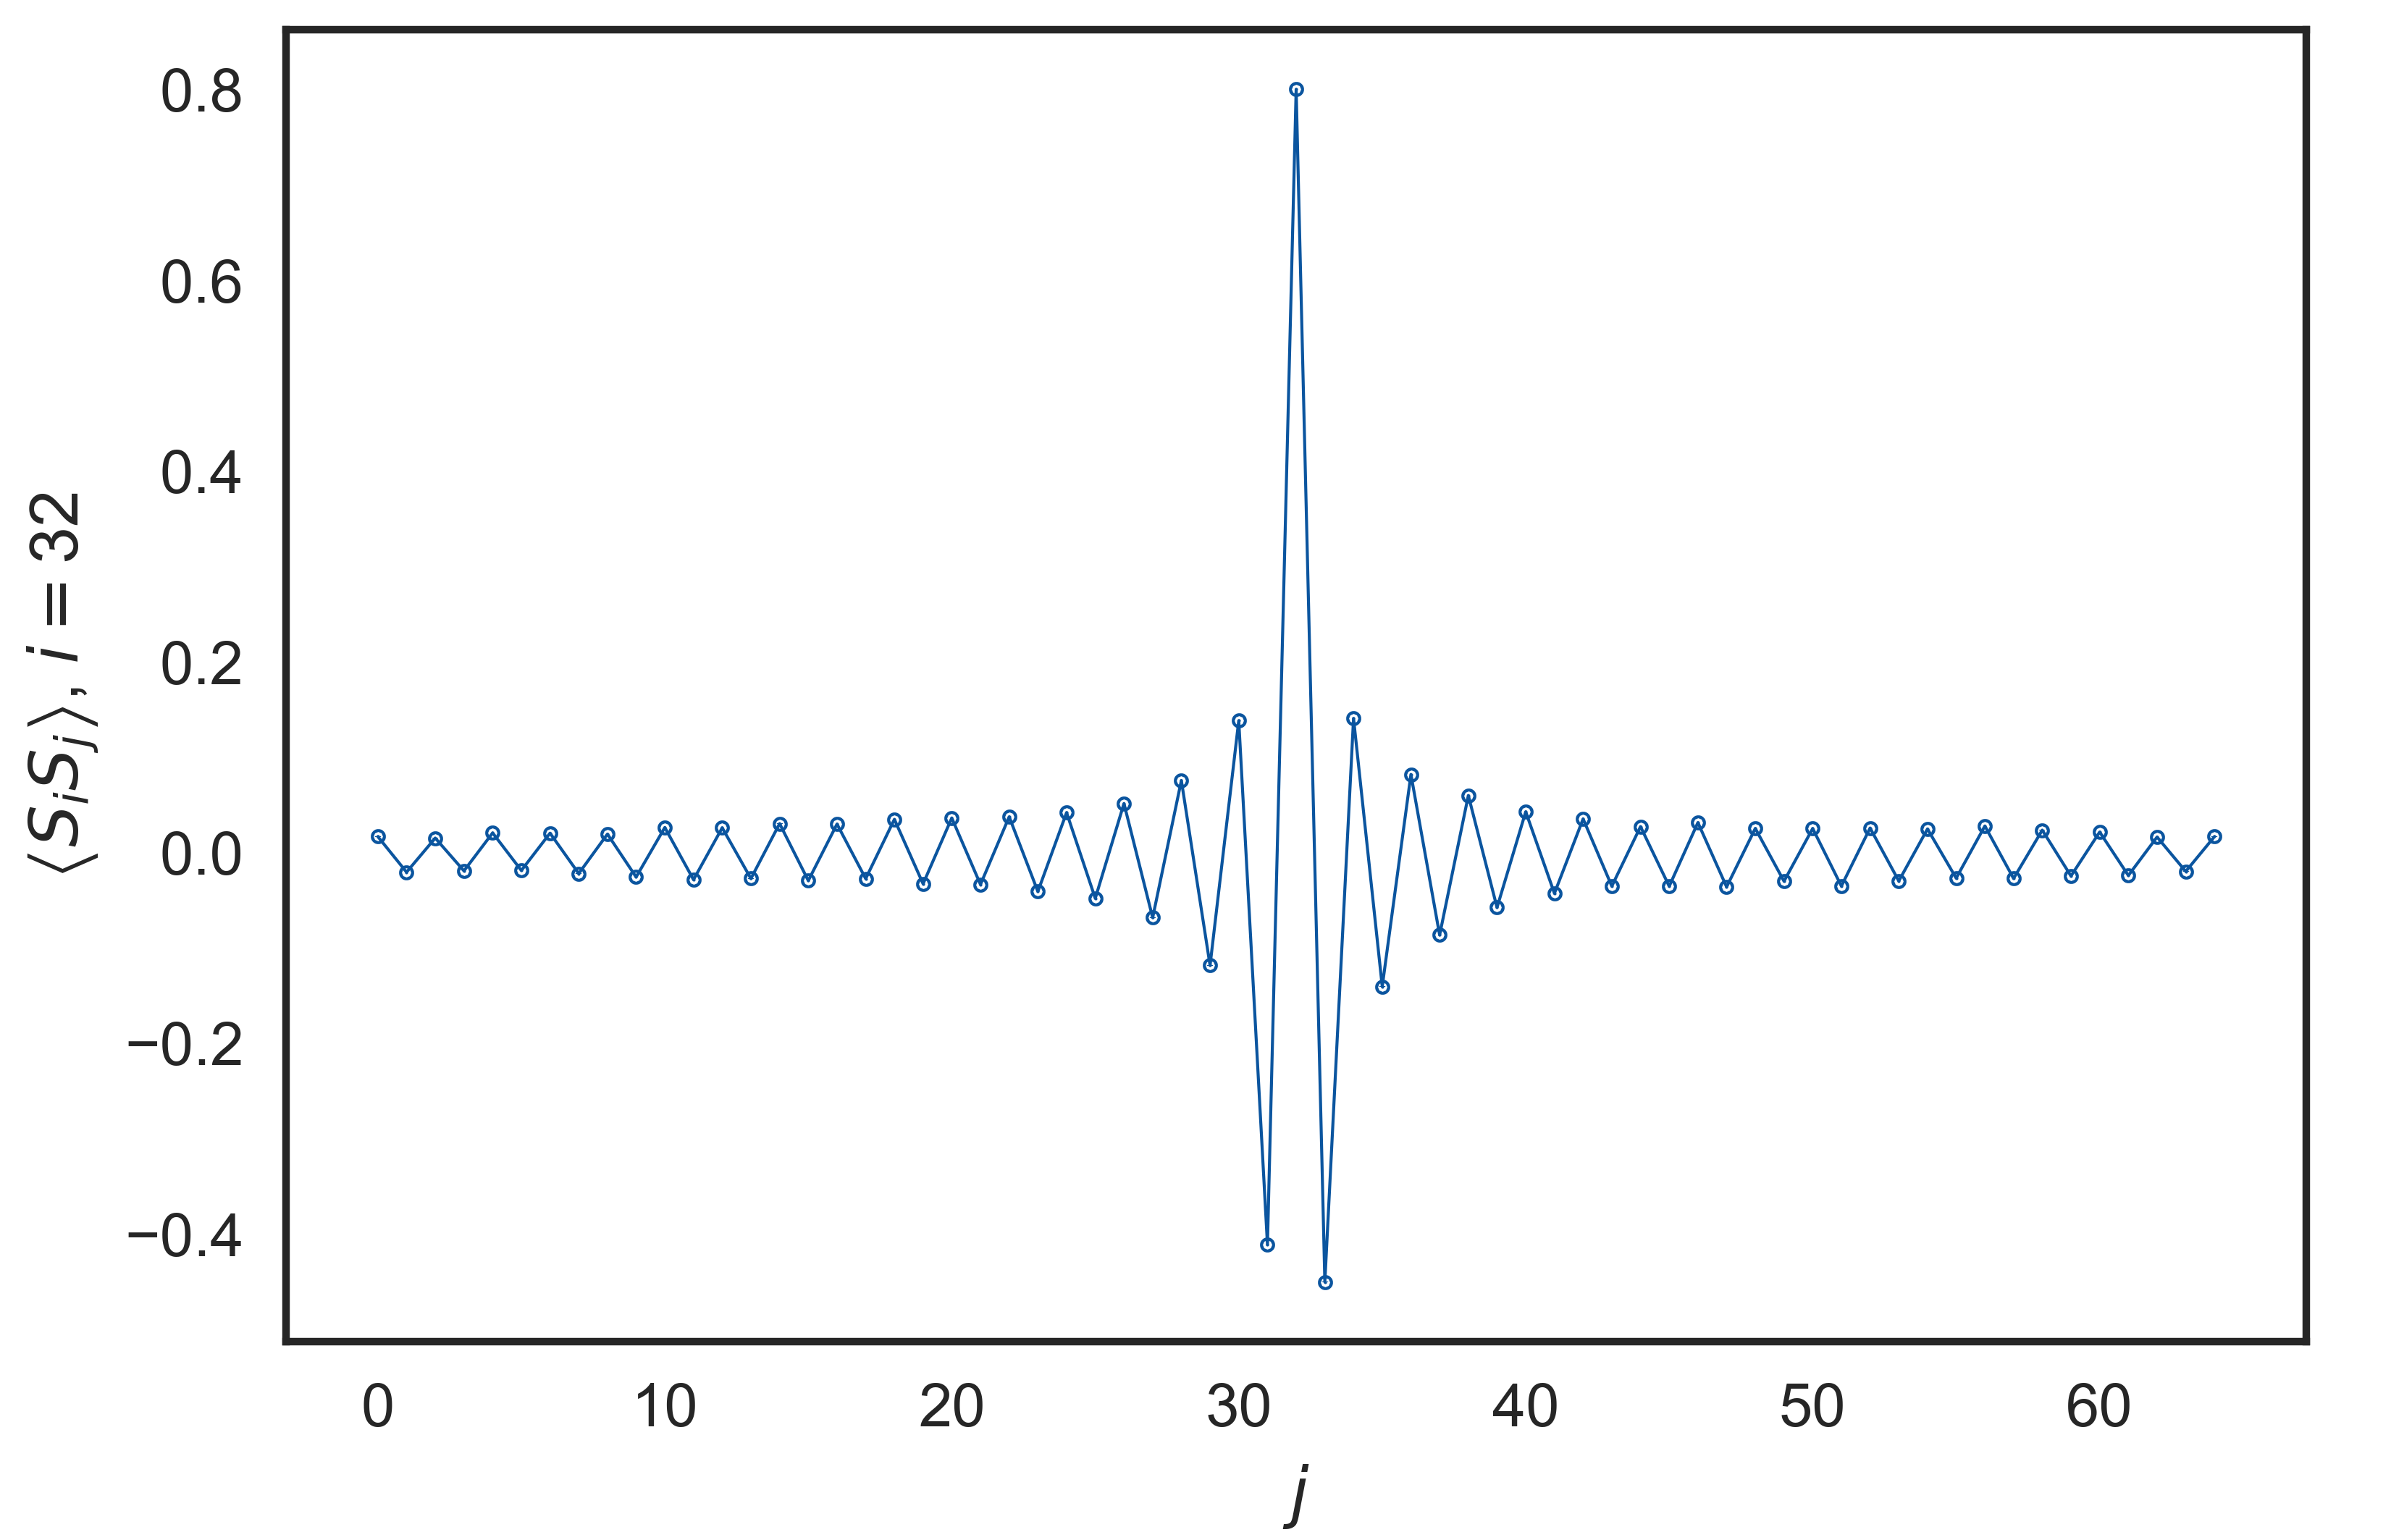
\includegraphics[scale=0.53]{Applications/magCorr.png}
\hspace{-0.5cm}
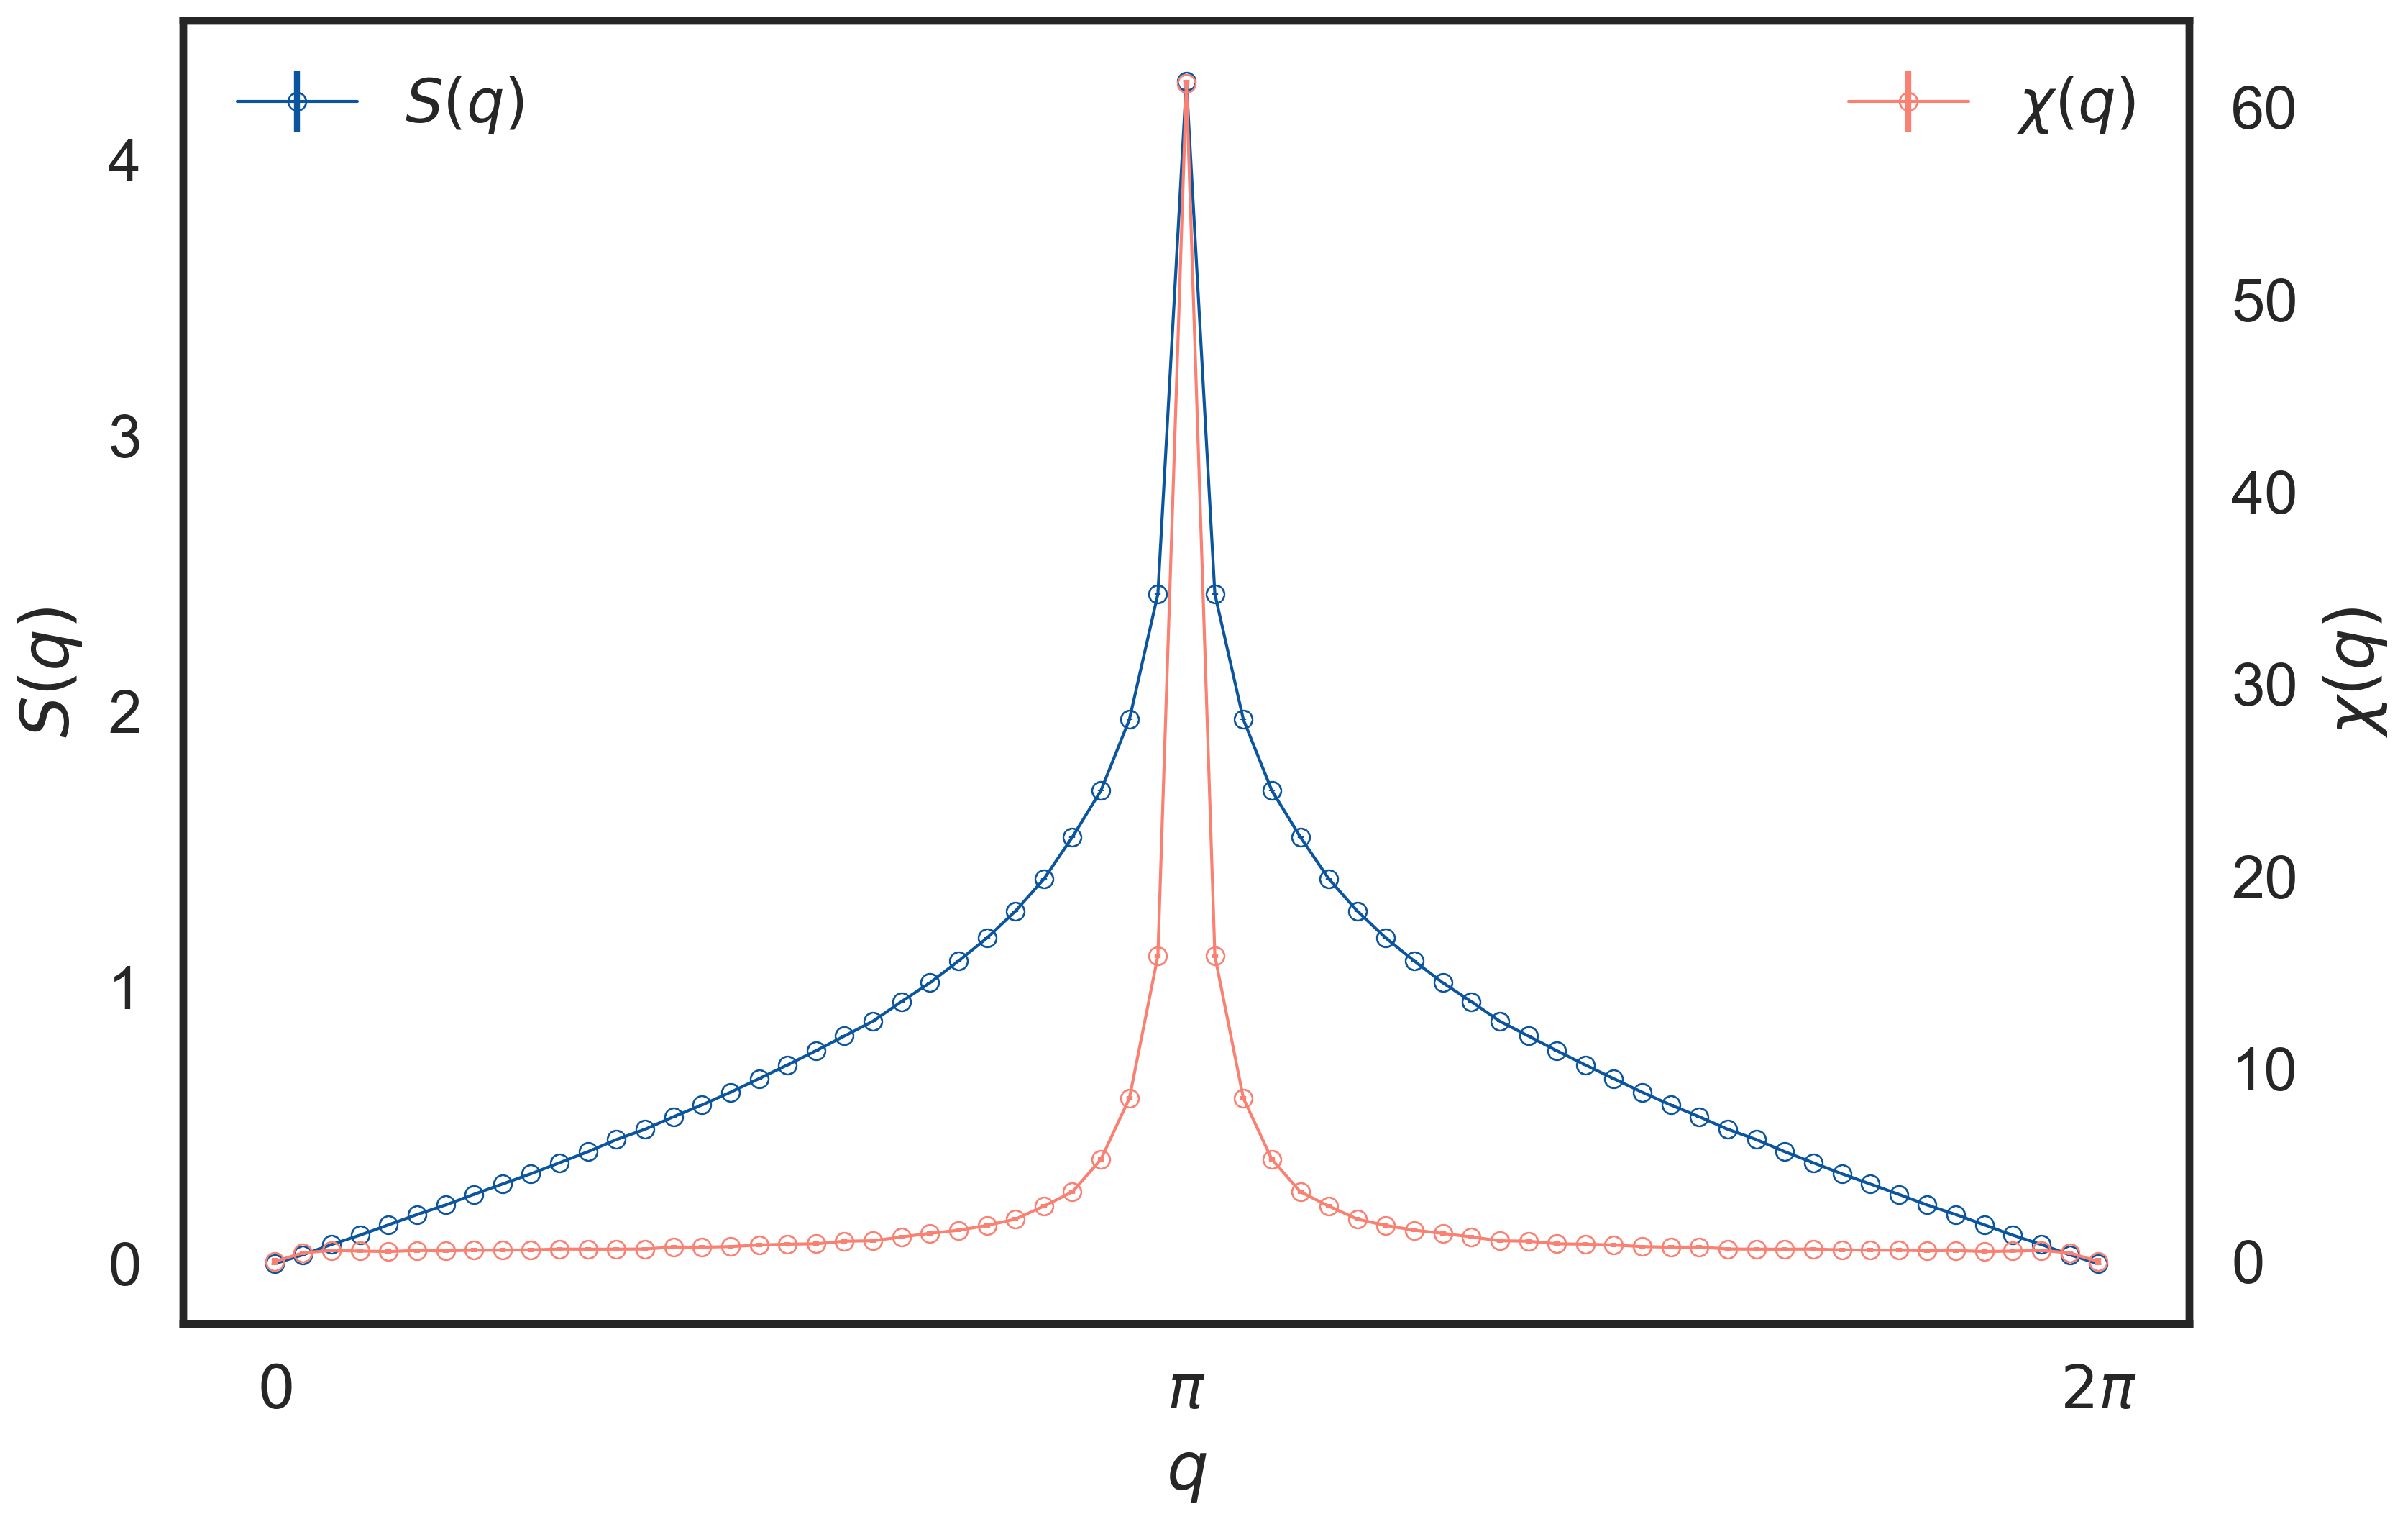
\includegraphics[scale=0.53]{Applications/SandChi.png}
\caption[Spin-spin correlation function, magnetic structure factor, and susceptibility for a 64 site Hubbard chain at $\beta = 25 t$, for $U = 4$.]{Spin-spin correlation function $\left\langle S^z_i S^z_j \right\rangle$ centered on the middle of the lattice (left); Magnetic structure factor, and susceptibility (right) for a 64 site Hubbard chain at $\beta = 25 t$, for $U = 4$, at half filling $\left\langle n \right\rangle = 1$.}
\end{figure}
\begin{figure}[H]\label{fig:Schi0}
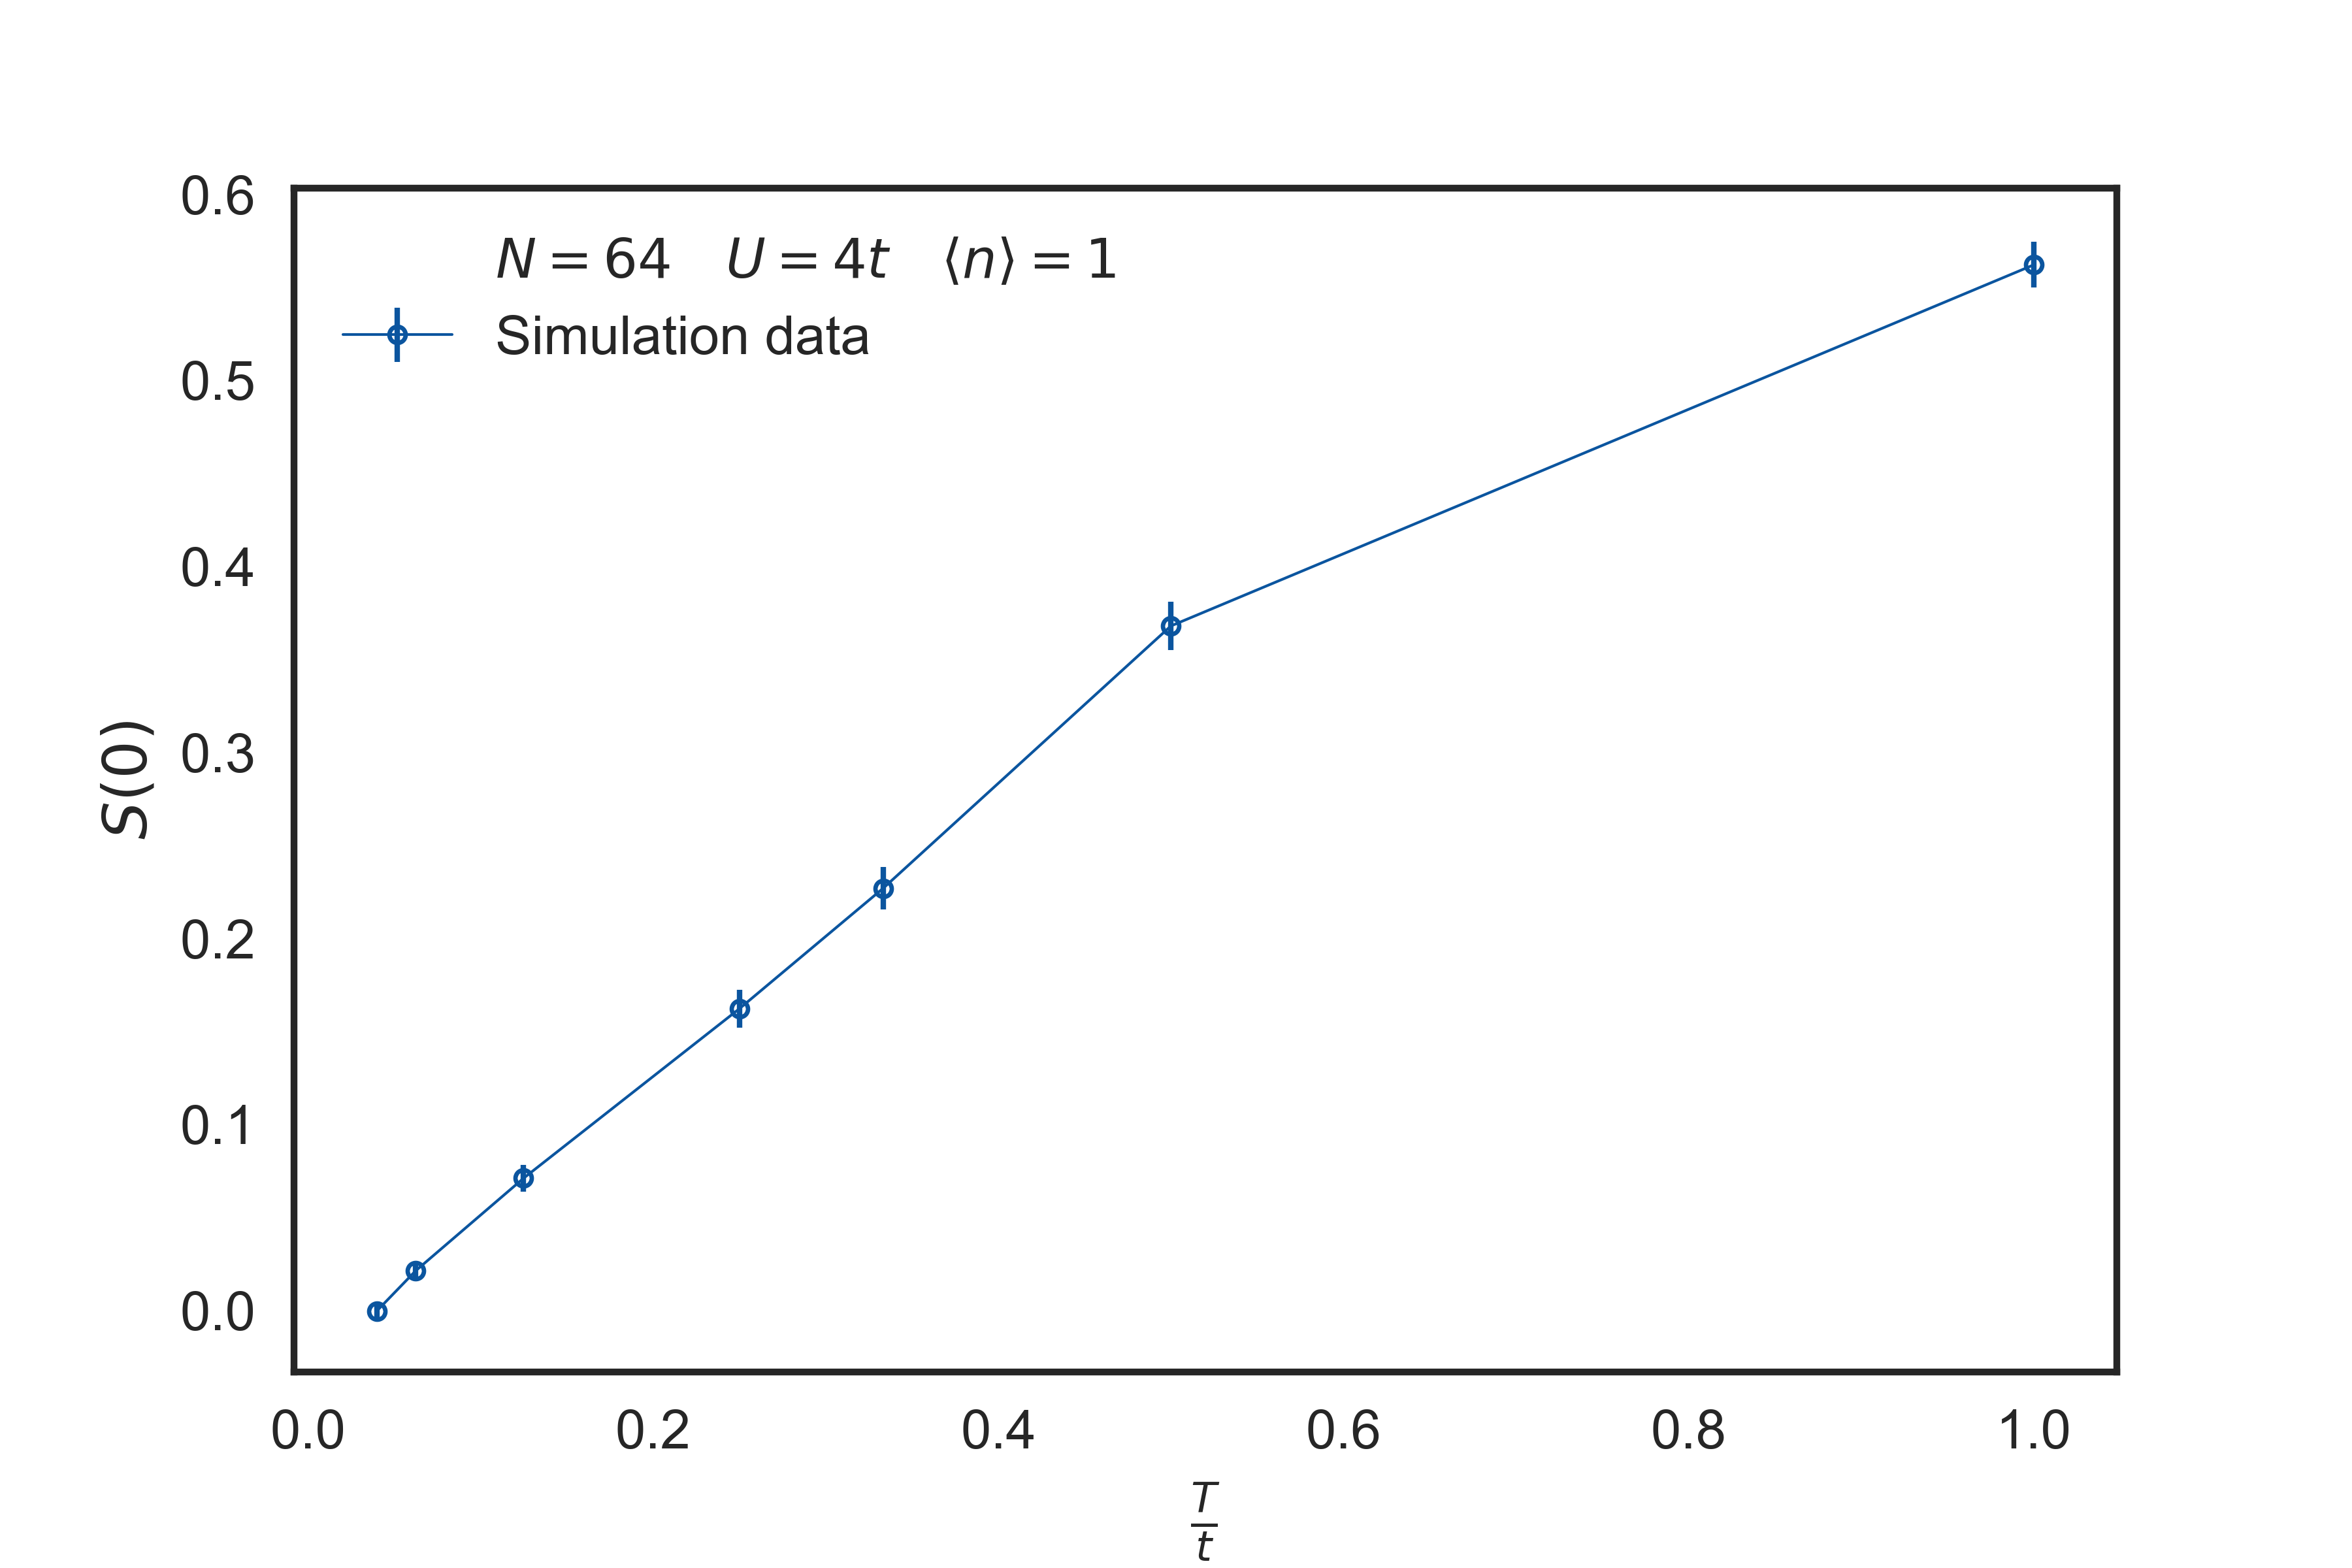
\includegraphics[scale=0.53]{Applications/S0T.png}
\hspace{-0.5cm}
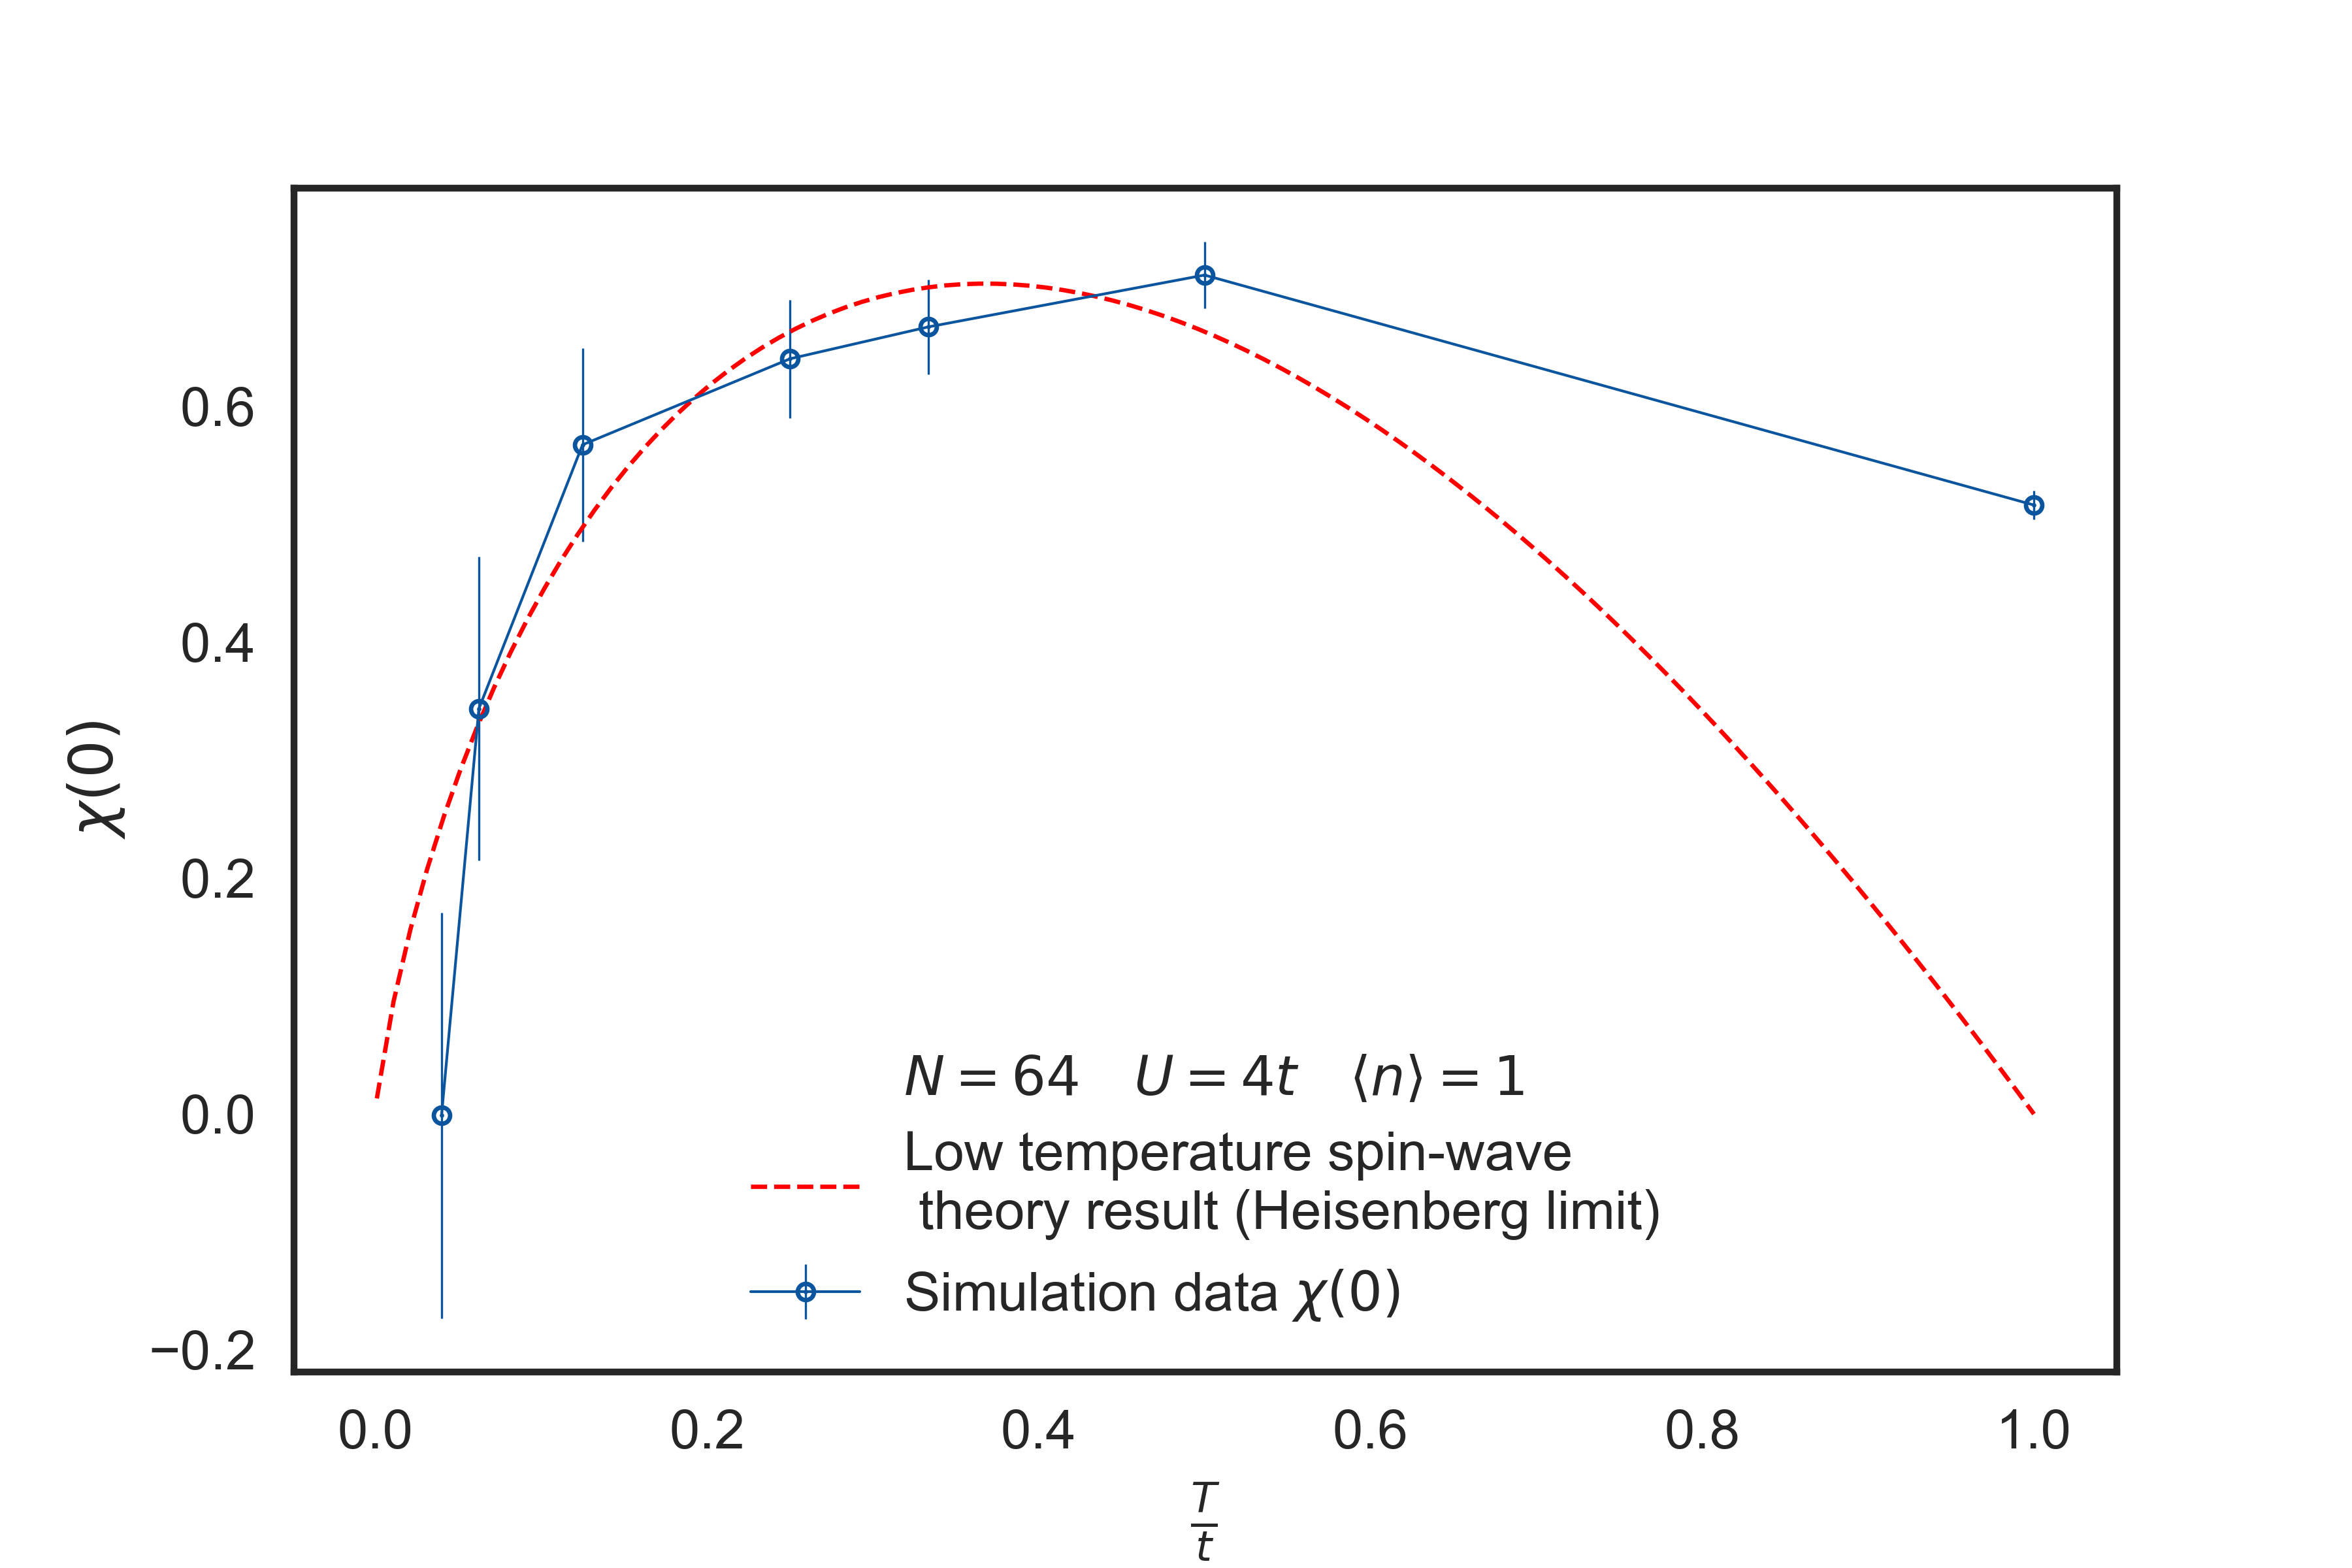
\includegraphics[scale=0.53]{Applications/Sus.png}
\caption[$q=0$ components of the magnetic structure factor and susceptibility as a function of temperature, indicating that the ground state does not have ferromagnetic ordering.]{$q=0$ components of the magnetic structure factor and susceptibility as a function of temperature, indicating that the ground state does not have ferromagnetic ordering.}
\end{figure}
\vspace{-0.5cm}
\begin{figure}[H]\label{fig:SchiPi}
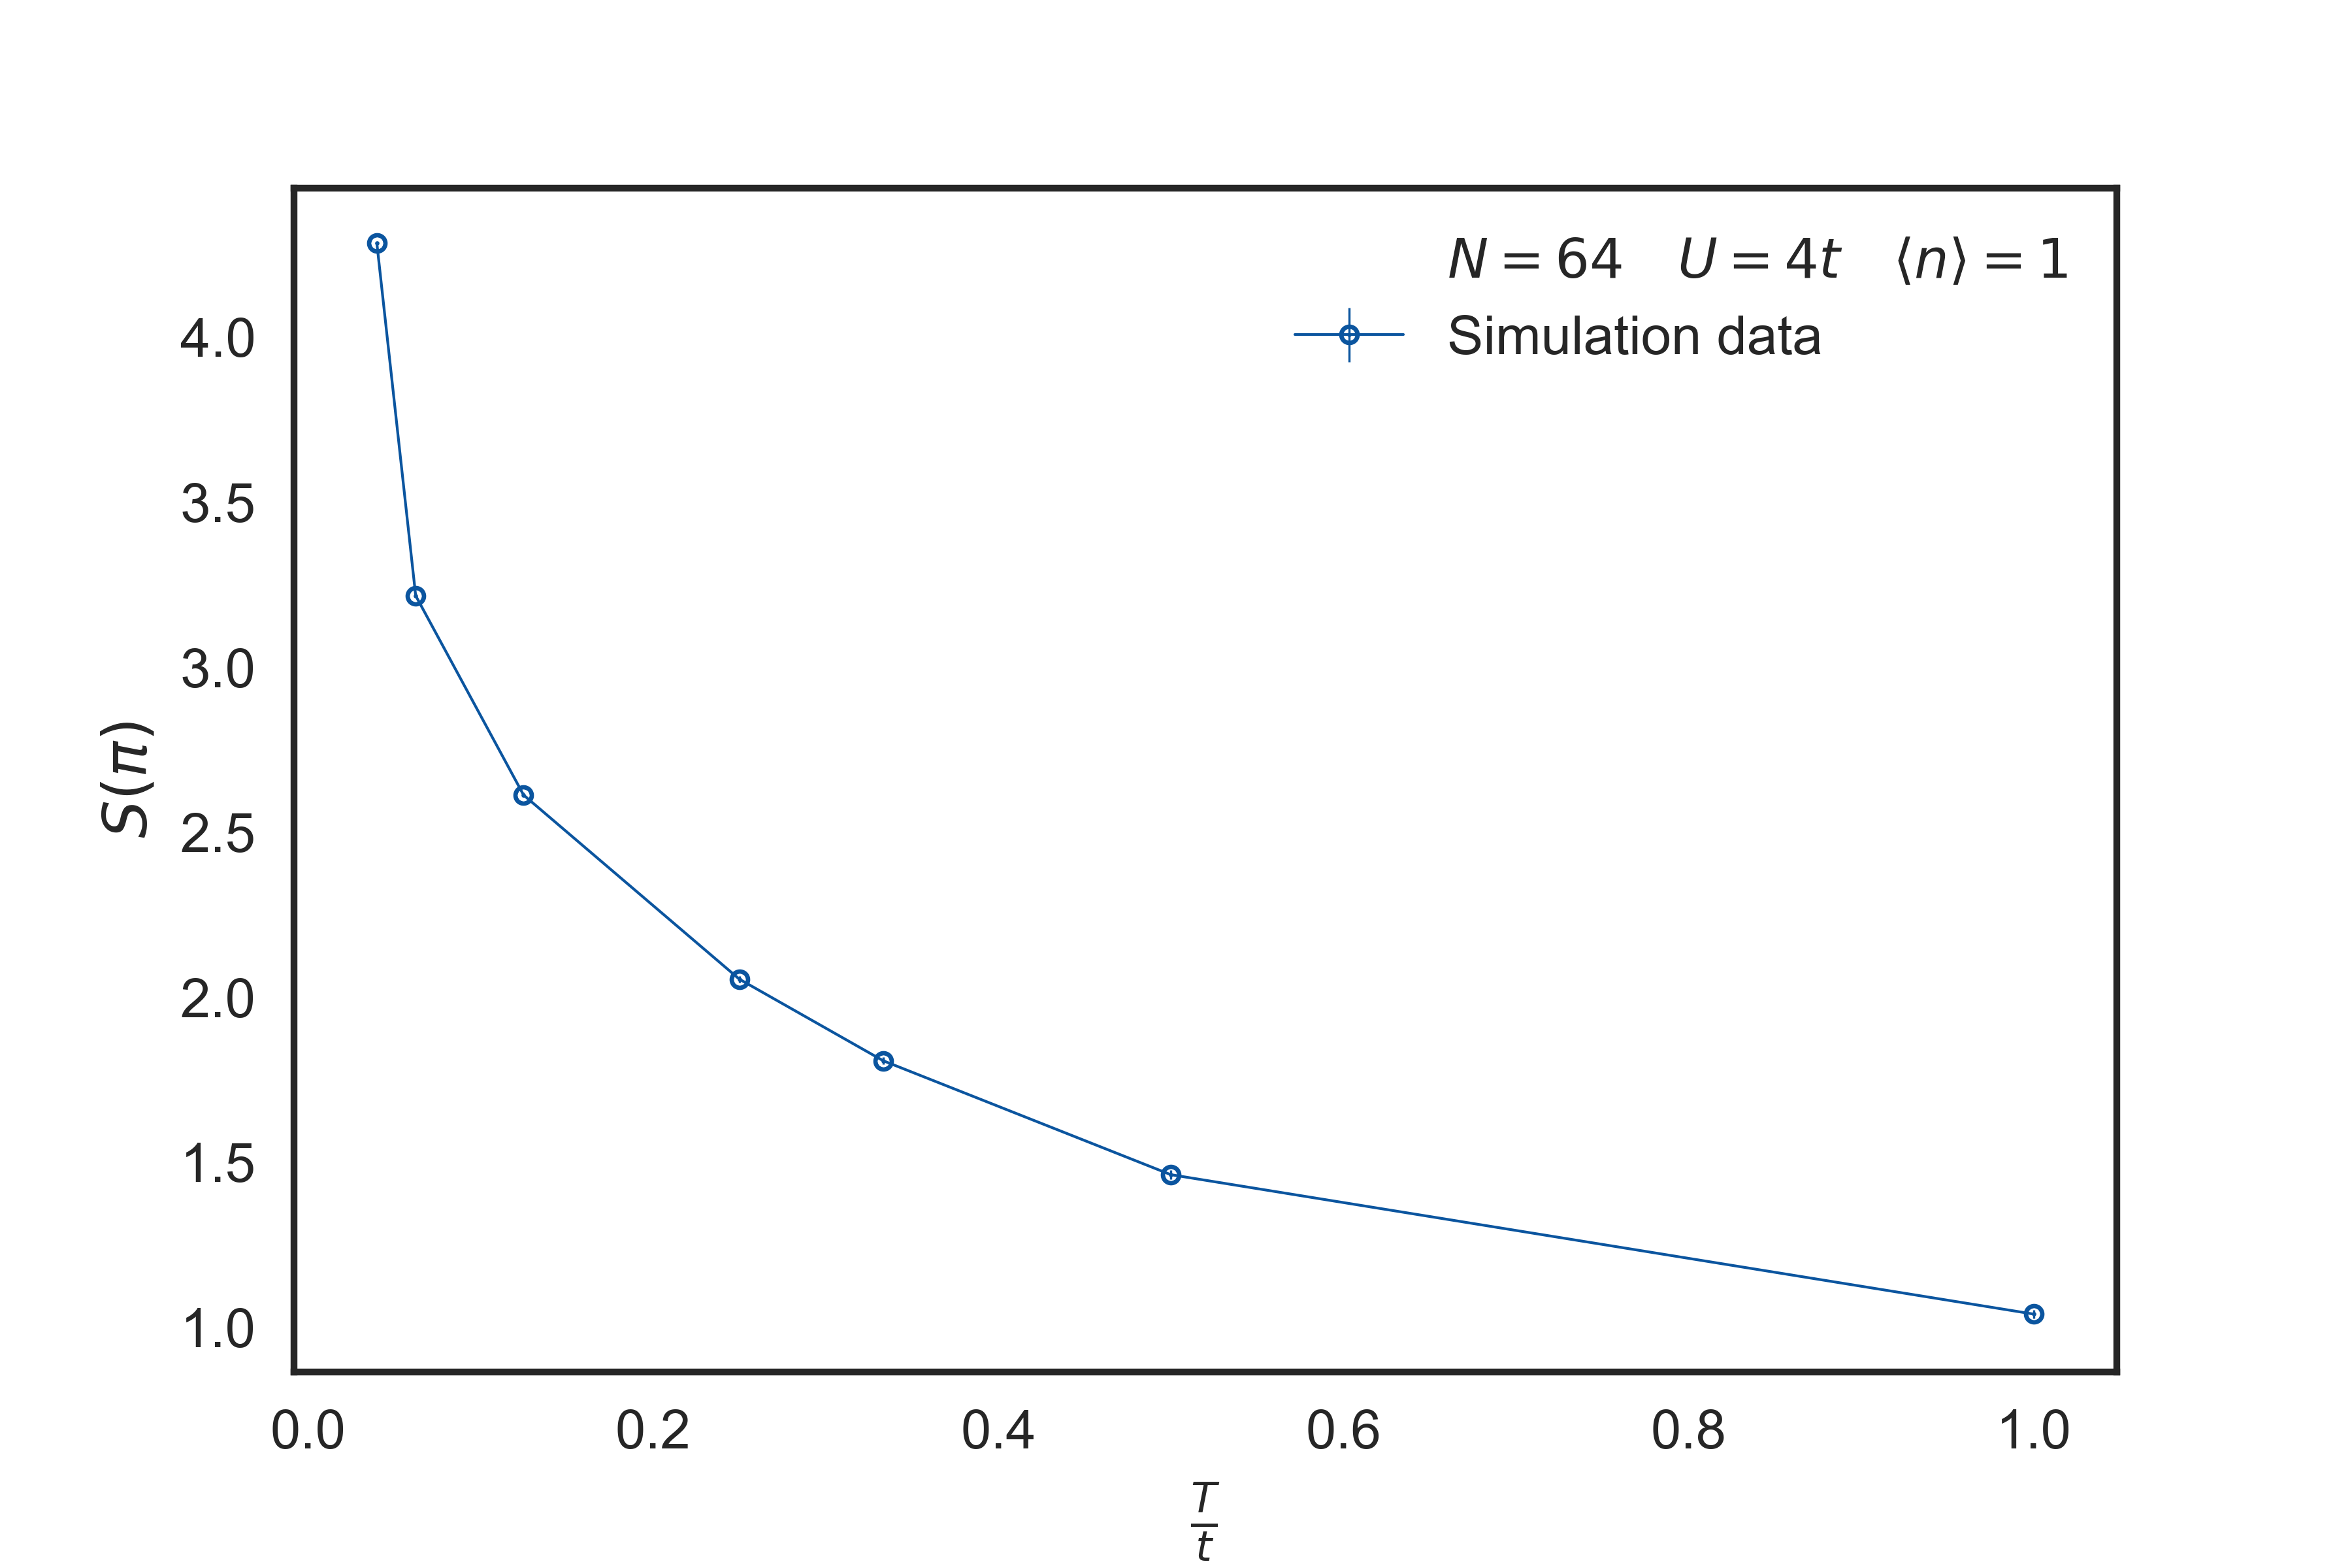
\includegraphics[scale=0.53]{Applications/SqT.png}
\hspace{-0.5cm}
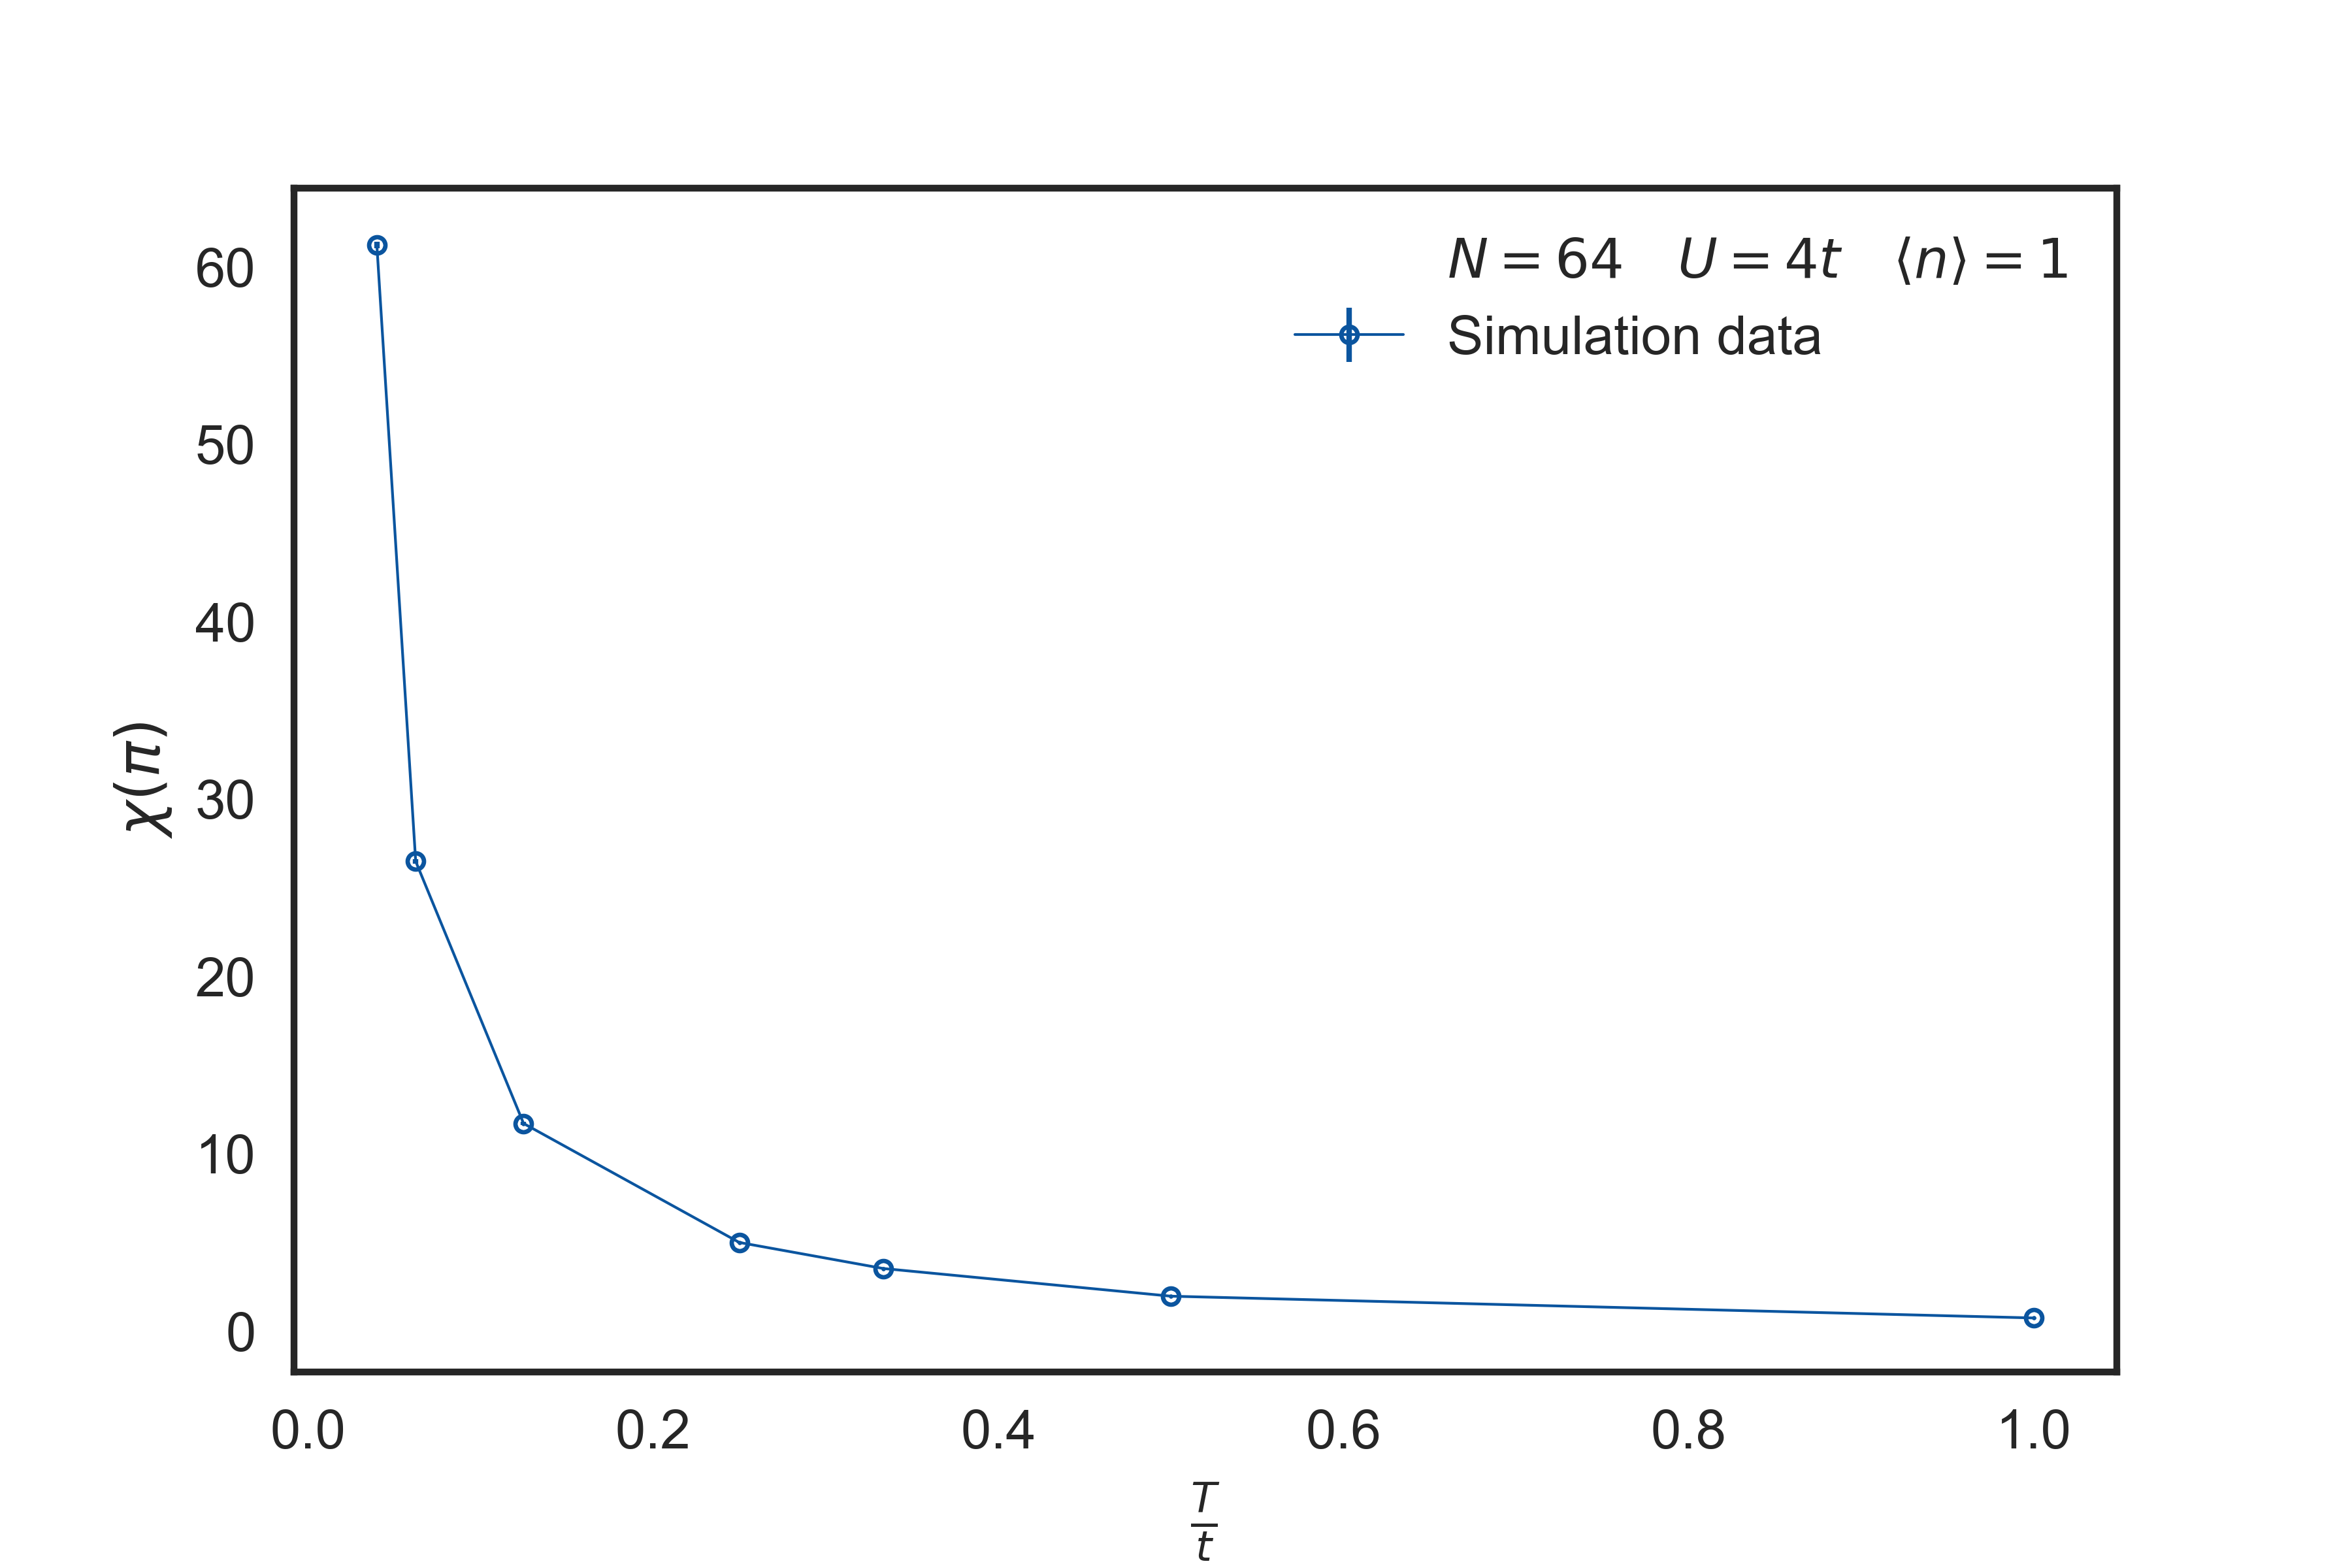
\includegraphics[scale=0.53]{Applications/stSus.png}
\caption[The magnetic structure factor and the  susceptibility have a peak at $q = \pi$ that increases as $T\rightarrow 0$, indicating \emph{antiferromagnetic ordering}.]{The magnetic structure factor and the susceptibility have a peak at $q = \pi$ that increases as $T\rightarrow 0$, indicating antiferromagnetic ordering.}
\end{figure}

We ran \texttt{QUEST} for the same 64-site chain as we did to obtain these results.
We used $\beta = 25 t$ and took half filling ($\left\langle n \right\rangle = 1$), and set $U = 4$, finding a remarkable agreement between the measurements obtained using our code and using \texttt{QUEST}.
Then, we took a small system to compare the run time and verify the $\mathcal{O}(L)$ scaling of the determinant \ac{QMC} algorithm.
We verify that \texttt{QUEST}'s algorithm sometimes suffers from large overhead time due to the pre-conditioning needed to stabilize matrix products.

\begin{figure}[H]\label{fig:quest_time}
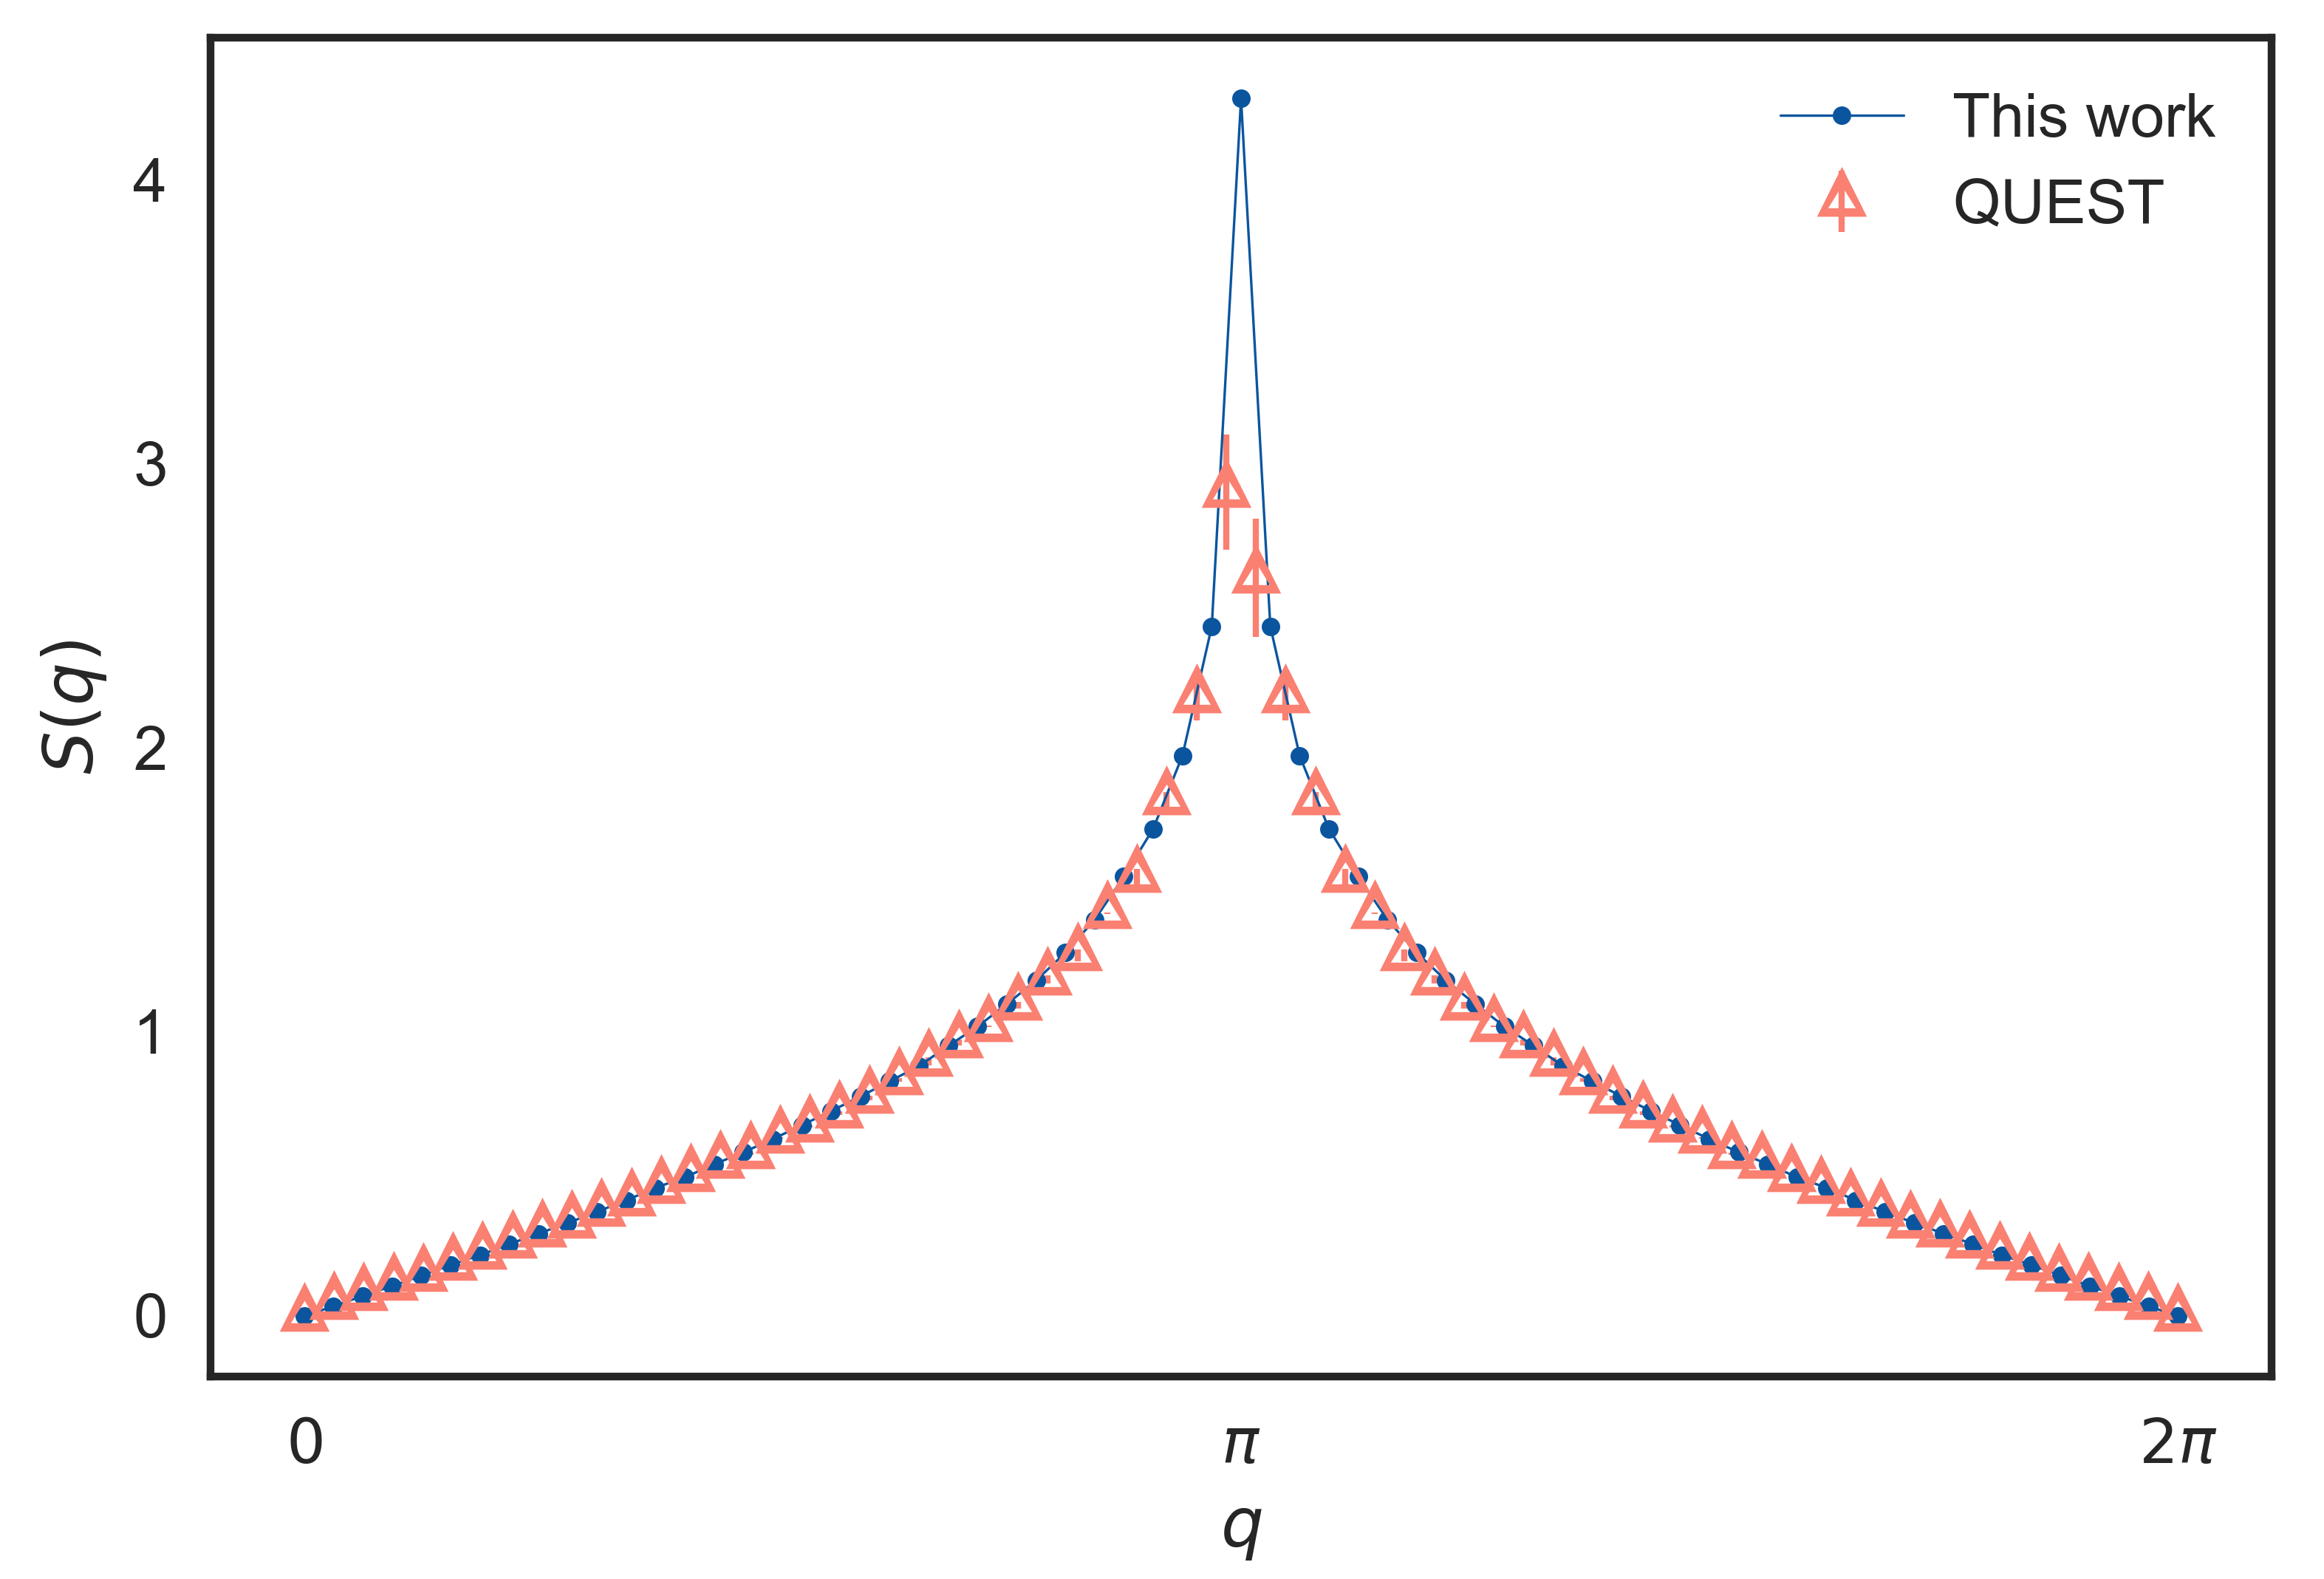
\includegraphics[scale=0.53]{Applications/s_compare.png}
\hspace{-0.5cm}
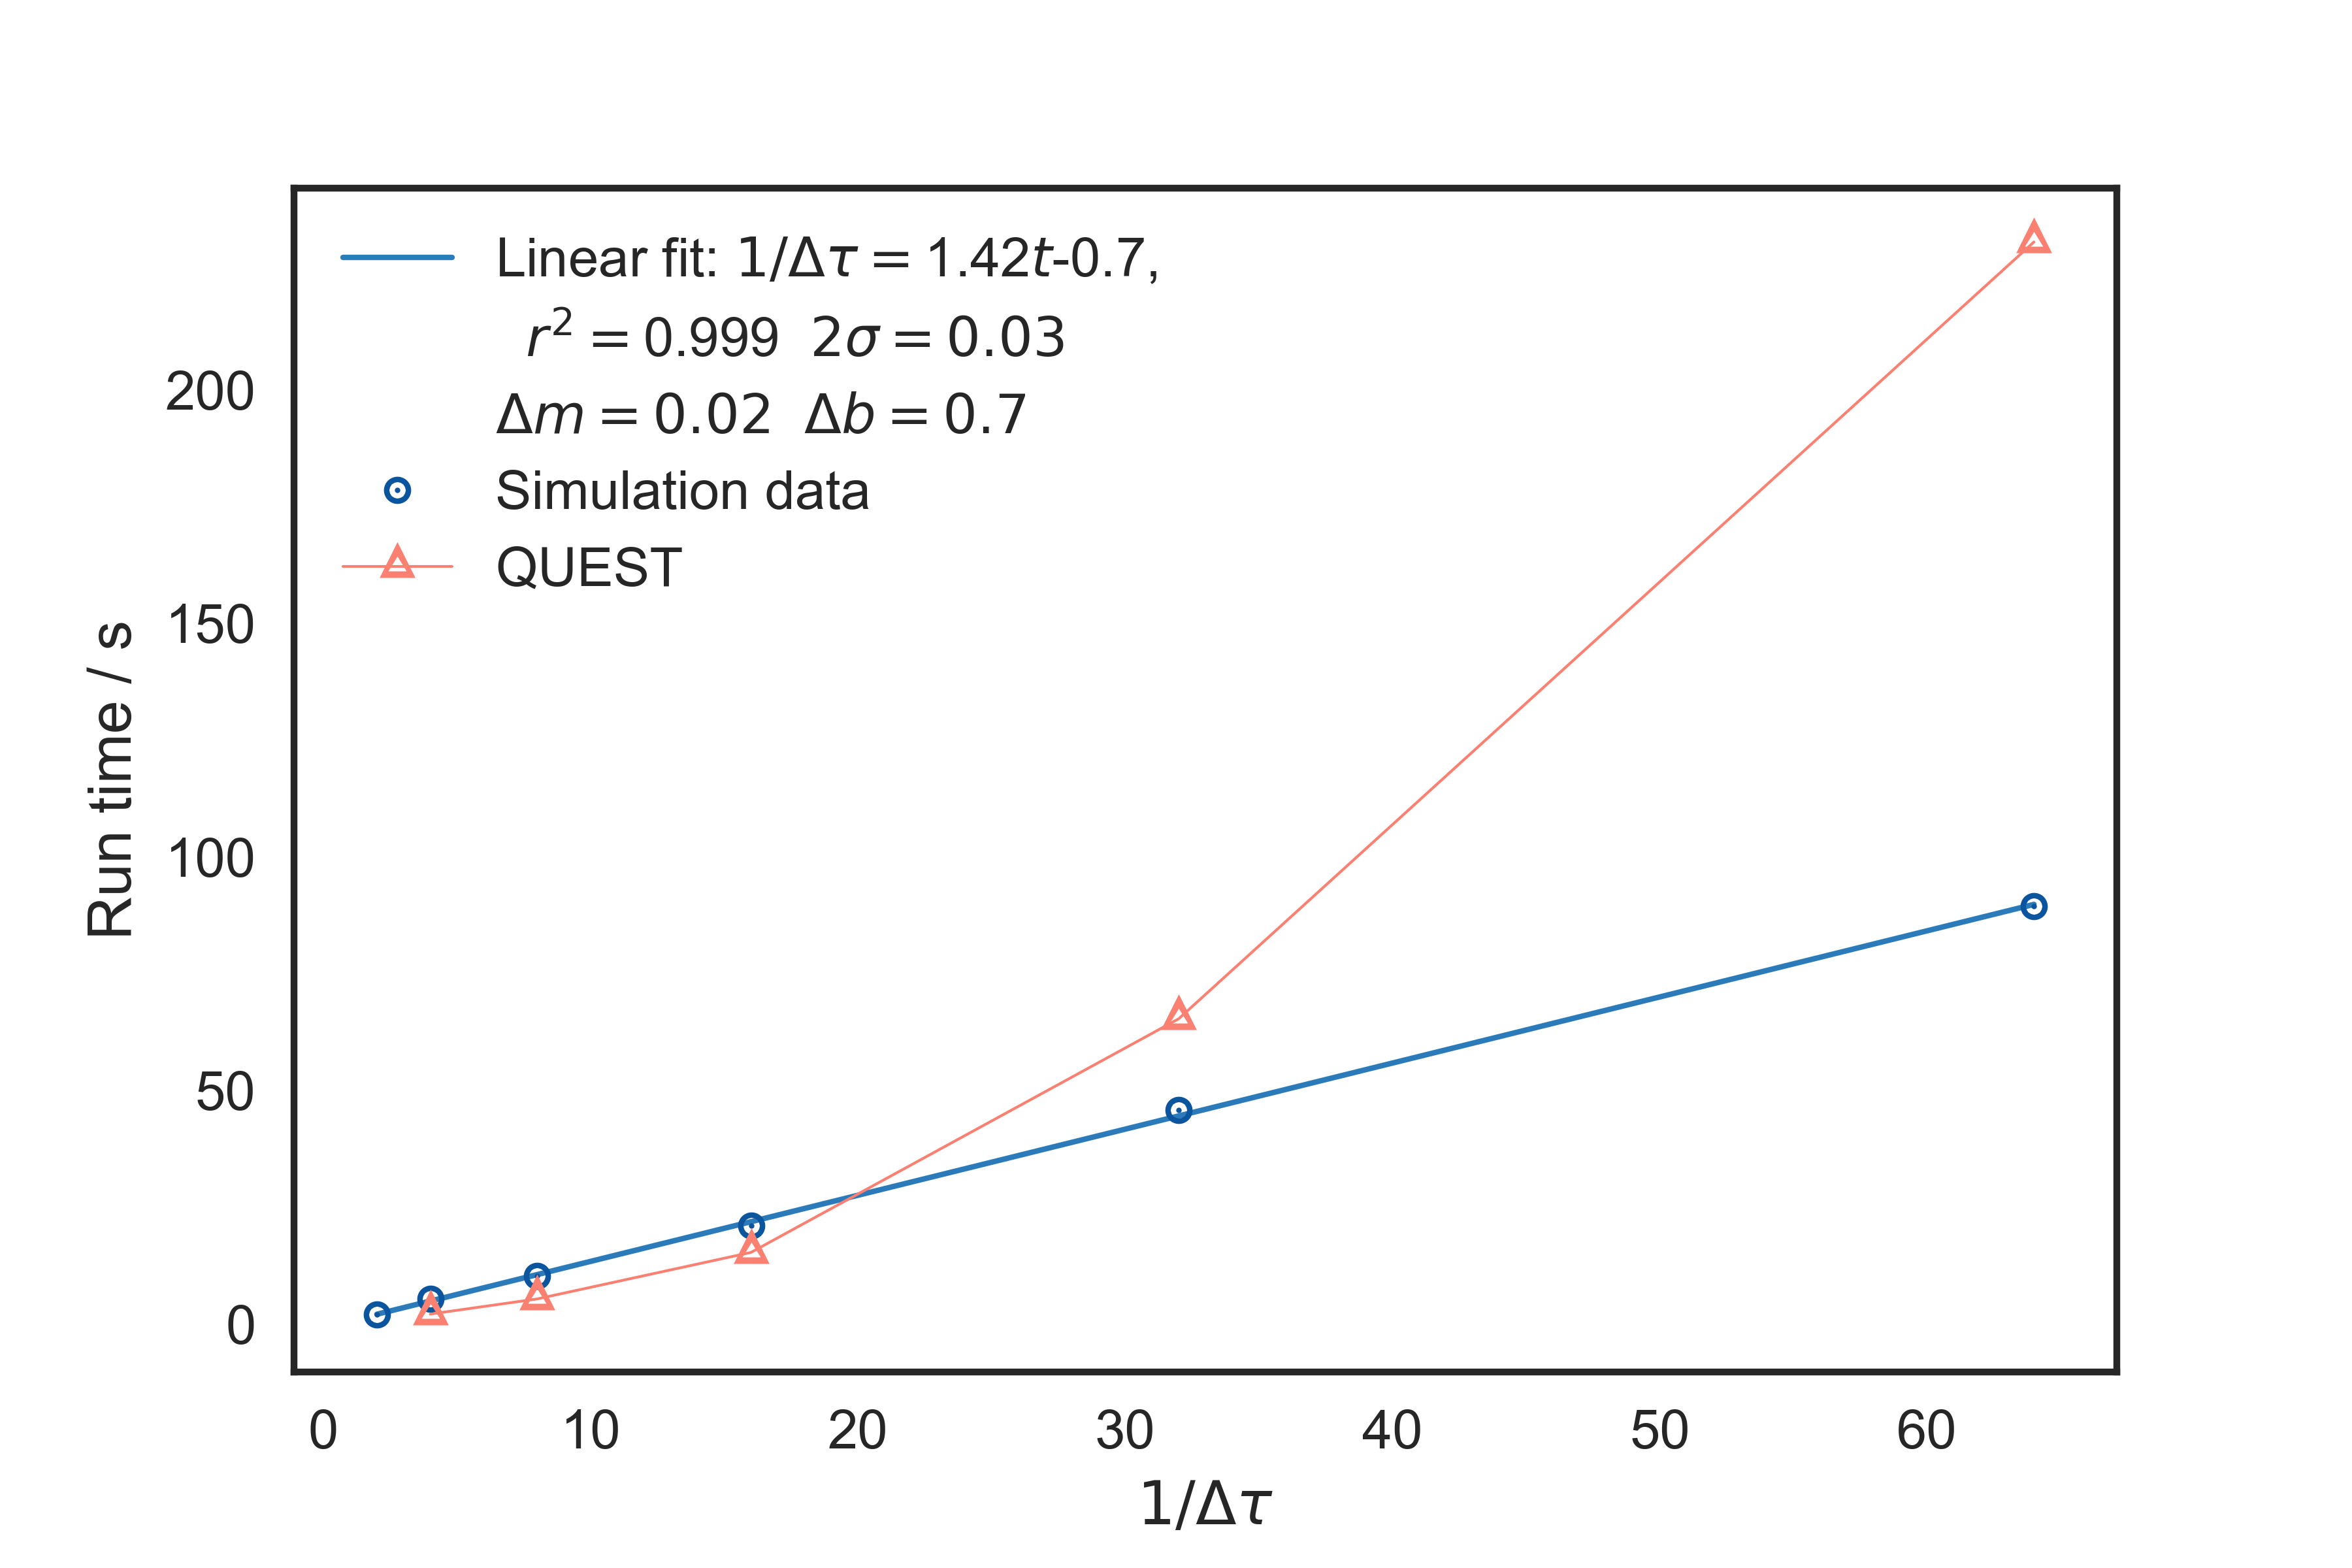
\includegraphics[scale=0.53]{Applications/runtime2sites.png}
\caption[Comparison of the magnetic structure factor with that obtained using \texttt{QUEST}. Run time comparison.]{Left: Comparison of the magnetic structure factor with that obtained using \texttt{QUEST}.
Right: The run time using our code increases linearly with $L$, as expected.
The \texttt{QUEST} algorithm initially increases linearly, but then becomes much slower due to the large overhead associated with pre-conditioning.}
\end{figure}
\vspace{-0.5cm}
\begin{figure}[H]\label{fig:hirsch1982}
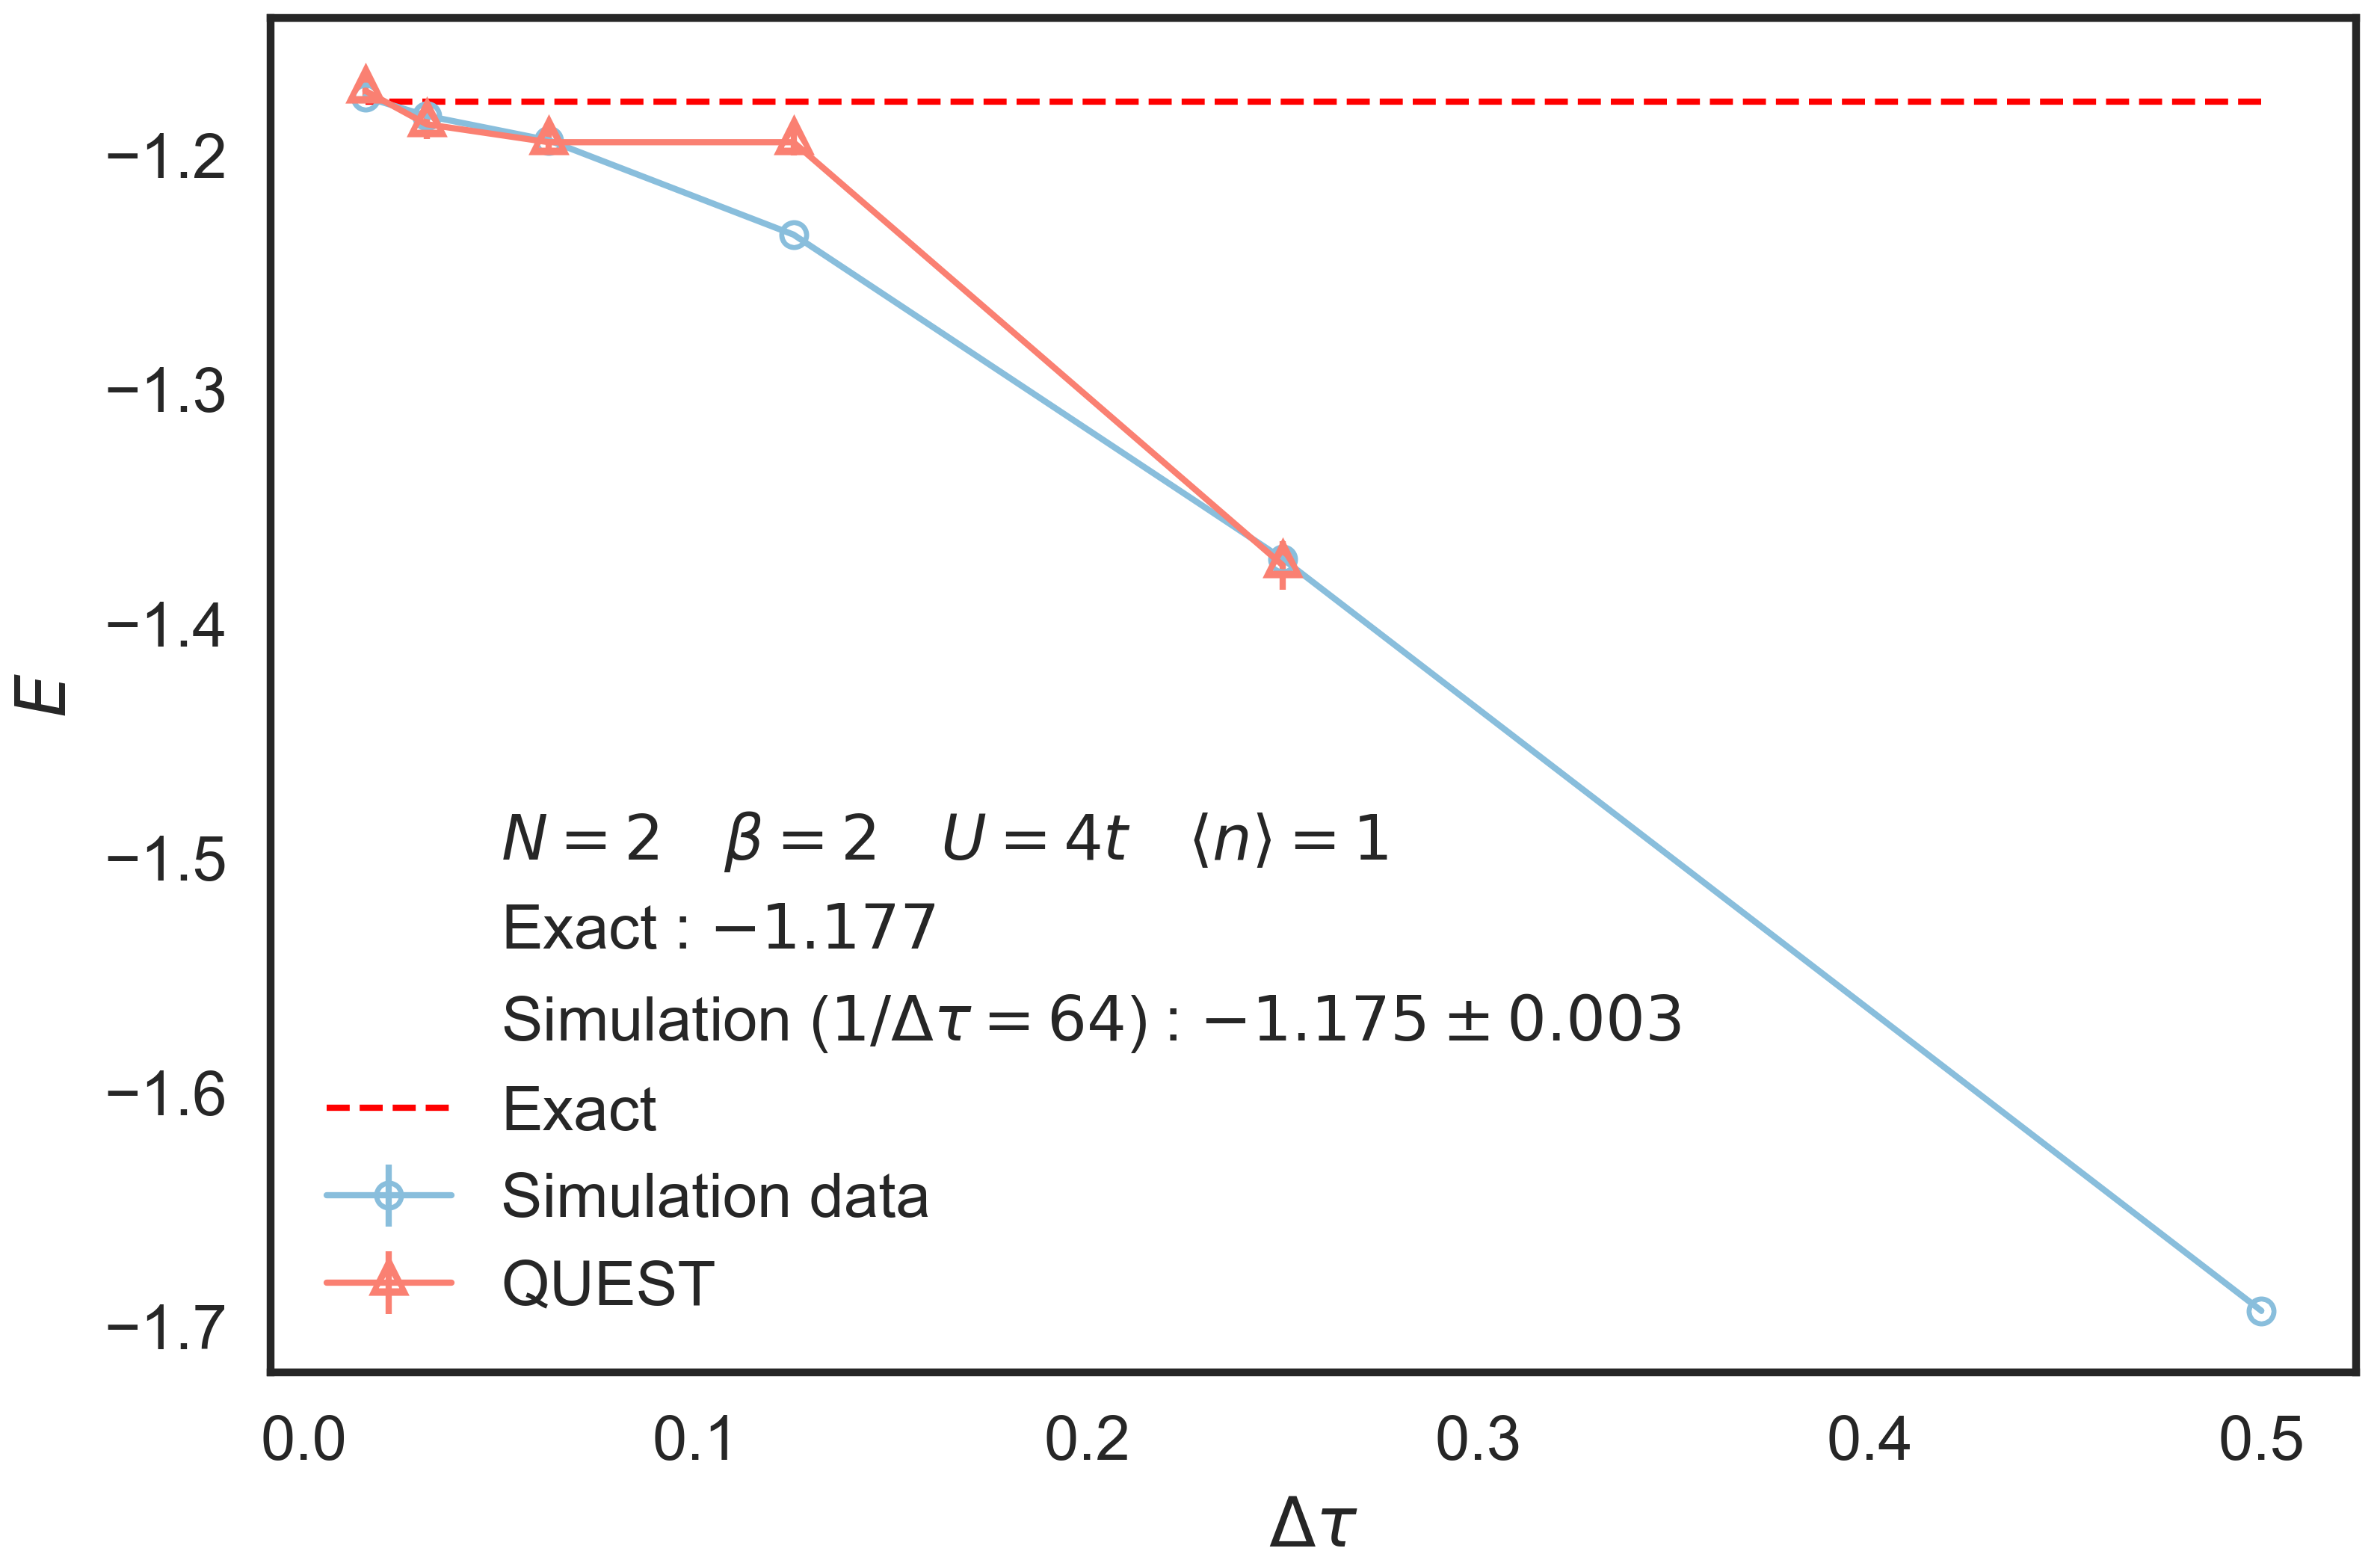
\includegraphics[scale=0.53]{Applications/Ehirsch1982.png}
\hspace{-0.5cm}
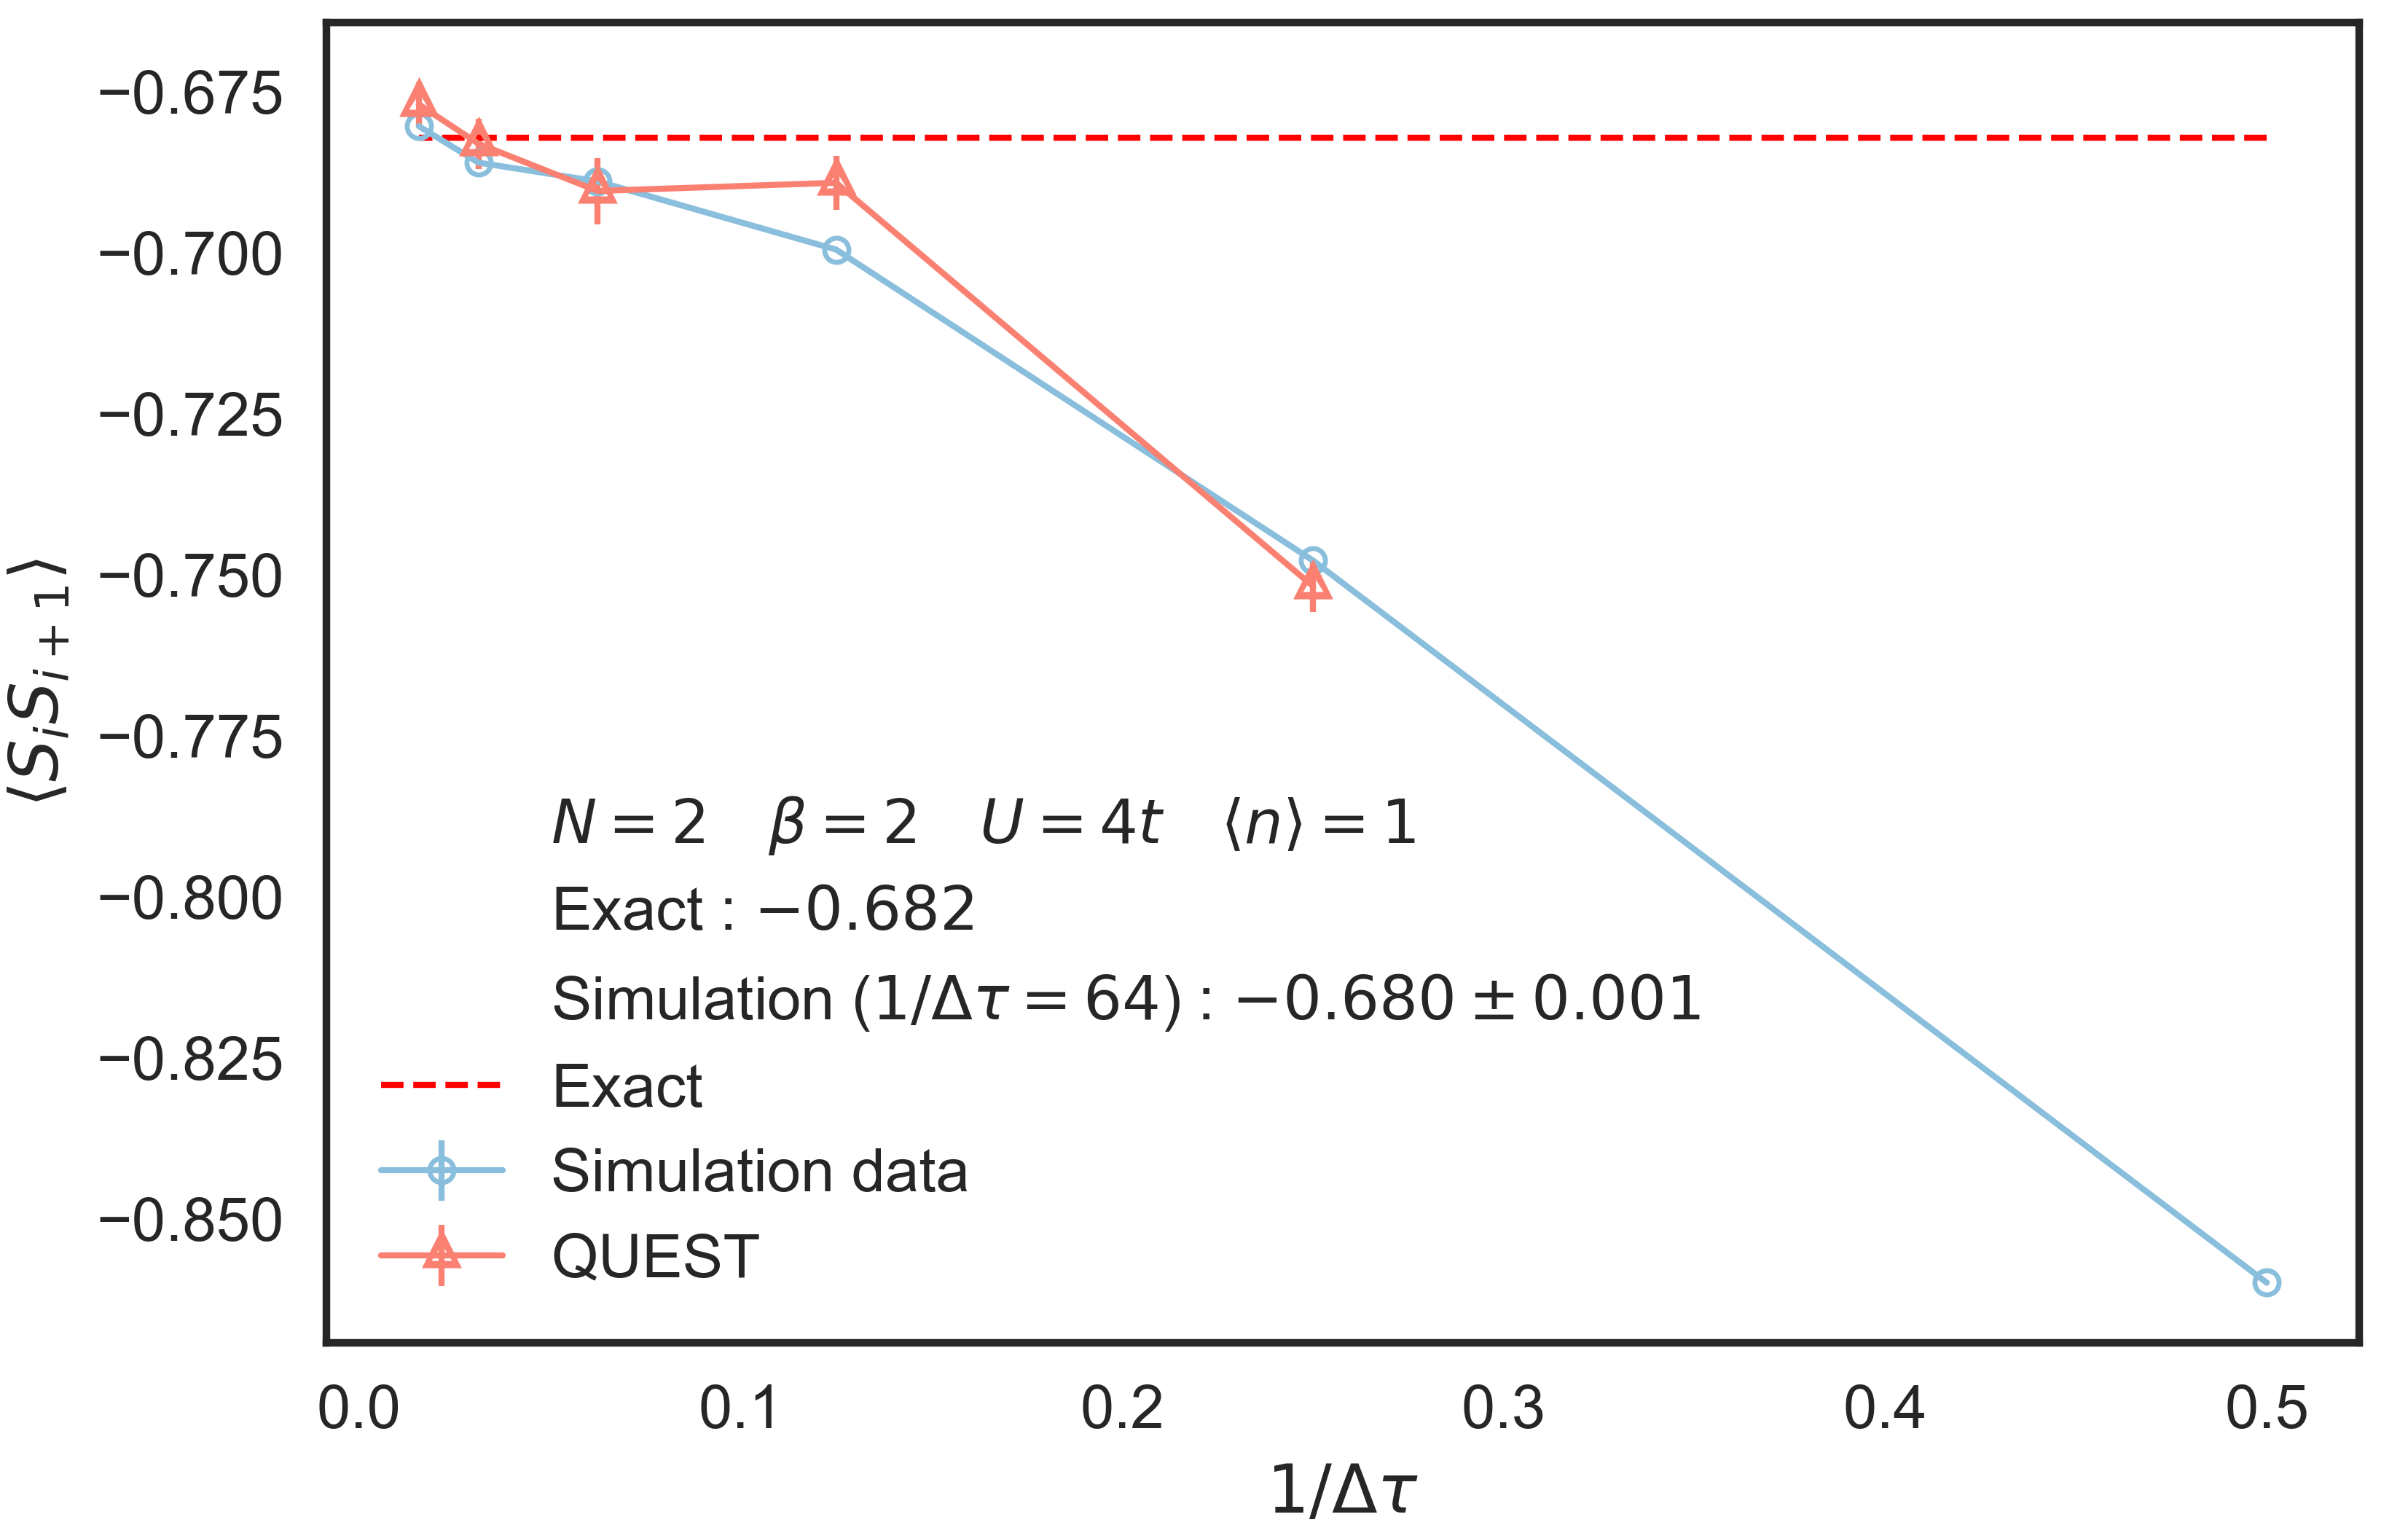
\includegraphics[scale=0.53]{Applications/SiSjhirsch1982.png}
\caption[]{Convergence of some of the measured observables to the exact value given by exact diagonalization for $N=2$, $\beta = 2 t$, $U = 4 t$}
\end{figure}
